\documentclass[conference, dvipsnames]{IEEEtran}

% Usepackages
\usepackage{cite}
% provides various features to facilitate writing math formulas and to improve the typographical quality of their output.
%\usepackage{amsmath}
\usepackage[cmex10]{amsmath}
\interdisplaylinepenalty=2500
\usepackage{amssymb,amsfonts}
\usepackage{algorithmic}
%\usepackage{graphicx}
\usepackage[dvips]{graphicx}
\usepackage{textcomp}
\usepackage{xcolor}

% formatting from IEEE conference. Needs to be fitted with our natbib
\def\BibTeX{{\rm B\kern-.05em{\sc i\kern-.025em b}\kern-.08em
		T\kern-.1667em\lower.7ex\hbox{E}\kern-.125emX}}

%%%%%%%%%%%%%%%%%%%%%%%%
%Article stuff
%%%%%%%%%%%%%%%%%%%%%%%%
% This package serves to balance the column lengths on the last page of the document.
% please, insert \balance command in the left column of the last page
\usepackage{balance}
\usepackage{supertabular}
\usepackage{paralist}
\usepackage{booktabs}
\usepackage{listings}


%Code listing style named "mystyle"
\lstdefinestyle{mystyle}{
	backgroundcolor=\color{white},   
	commentstyle=\color{olive},
	keywordstyle=\color{purple},
	numberstyle=\tiny\color{gray},
	stringstyle=\color{blue},
	basicstyle=\ttfamily\footnotesize,
	breakatwhitespace=false,         
	breaklines=true,                 
	captionpos=b,                    
	keepspaces=true,                 
	numbers=left,                    
	numbersep=5pt,                  
	showspaces=false,                
	showstringspaces=false,
	showtabs=false,                  
	tabsize=2
}

%"mystyle" code listing set
\lstset{style=mystyle}


% Coloring stuff
\usepackage{xcolor}
\usepackage[most]{tcolorbox}
\usepackage[english]{babel}
\usepackage{wrapfig}
\newcommand{\thiscolor}[1]{\colorbox{#1}{\phantom{Here is text}}}
\newcommand{\mycolor}[3]{
	\!\!\!\!\! \tcbox[sharp corners, size=small,
	colback=#1, colframe=white, 
	halign upper=left, valign upper=top,
	halign lower=right, valign lower=bottom,
	enhanced, on line, boxsep=2pt,
	underlay = {
		\begin{tcbclipinterior}
			\filldraw[fill=#2, draw=tcbcolframe] (frame.south west)--++(90:1cm) to [out=5, in=185] ([yshift=-1cm]frame.north east)|-cycle;
		\end{tcbclipinterior}
	}]{#3}}


%% to enable \thank command
\IEEEoverridecommandlockouts 
% to typeset algorithms
\usepackage{algorithm}
%\usepackage{algpseudocode}
% to typeset code fragments
\usepackage{listings}
% to make an accent \k be available
\usepackage[T1]{fontenc}
% por urls typesetting and breaking
\usepackage{url}
% for vertical merging table cells
\usepackage{multirow}
\usepackage{siunitx}


%%%%%%%%%%%%%%%%%%%%%%%%
%Mixed packages
%%%%%%%%%%%%%%%%%%%%%%%%
\usepackage[hidelinks]{hyperref}
\usepackage{graphicx}
\usepackage[textsize=scriptsize]{todonotes}
\usepackage{glossaries}
\usepackage[numbers]{natbib}
\usepackage{subcaption}
\bibliographystyle{plainnat}

\let\labelindent\relax %Needed before enumitem to avoid error with IEEE template
\usepackage{enumitem}
% Encoding %
\usepackage[utf8]{inputenc}
\usepackage{enumitem}
\usepackage{framed}


%%%%%%%%%%%%%%%%%%%%%%%%
%Figures
%%%%%%%%%%%%%%%%%%%%%%%%

\usepackage{tikz}
\usepackage{pgfplots}

% Tables %
\usepackage{tabularx}
\usepackage{xltabular}
\newcolumntype{Y}{>{\centering\arraybackslash}X}
\usepackage{booktabs} % for professional tables
\usepackage{tikz}
\usetikzlibrary{positioning}
\usepackage{longtable}
\usepackage{makecell}
\usetikzlibrary{shapes.geometric, arrows}
\usetikzlibrary{matrix,positioning,arrows.meta,arrows}

\tikzset{my arrow/.style={-latex},
	set@com@col/.style={},set@com@col@aryarg/.style={column #1/.style={set@com@col}},
	set@com@row/.style={},set@com@row@aryarg/.style={row #1/.style={set@com@row}},
	set common column/.style 2 args={set@com@col/.style={#2}, set@com@col@aryarg/.list={#1}},
	set common row/.style 2 args={set@com@row/.style={#2}, set@com@row@aryarg/.list={#1}},
}

%%%%%%%%%%%%%%%%%%%%%%%%
%Defines
%%%%%%%%%%%%%%%%%%%%%%%%

\newtheorem{definition}{\textbf{Definition}}

% Autoref
\def\sectionautorefname{Section}
\def\subsectionautorefname{Section}
\def\subsubsectionautorefname{Section}
\def\figureautorefname{Fig.}
\def\definitionautorefname{Definition}

% Plates
\usepackage{amstext}
\usepackage{tikz}
\usetikzlibrary{arrows,decorations.pathmorphing,fit,positioning}

\newcommand{\dir}{\text{Dirichlet}}
\newcommand{\mult}{\text{Multinomial}}


% Macros
\input{setup/macros.tex}

% Glossaries
\input{setup/acronyms.tex}


\begin{document}
% Autoref
\def\sectionautorefname{Section}
\def\subsectionautorefname{Section}
\def\subsubsectionautorefname{Section}
%\def\figureautorefname{Fig.}
\def\definitionautorefname{Definition}

\title{Very Incredibly Complex Title\\
%\thanks{Identify applicable funding agency here. If none, delete this.}
}

%\IEEEauthorblockN{Dennis Højbjerg Rose, Peter Langballe Erichsen, and Rasmus Engesgaard Christensen}\\
%\IEEEauthorblockA{Department of Computer Science, Aalborg University,\\Selma Lagerløfs Vej 300, 9220 Aalborg Øst, Denmark\\Email: \{drose16, perich16, rech16\}@student.aau.dk}}

\author{
\IEEEauthorblockN{Dennis Højbjerg Rose}
\IEEEauthorblockA{\textit{Department of Computer Science} \\
\textit{Aalborg University}\\
Aalborg, Denmark \\
drose16@student.aau.dk}
\and
\IEEEauthorblockN{Peter Langballe Erichsen}
\IEEEauthorblockA{\textit{Department of Computer Science} \\
\textit{Aalborg University}\\
Aalborg, Denmark \\
perich16@student.aau.dk}
\and
\IEEEauthorblockN{Rasmus Engesgaard Christensen}
\IEEEauthorblockA{\textit{Department of Computer Science} \\
\textit{Aalborg University}\\
Aalborg, Denmark \\
rech16@student.aau.dk}
}

\maketitle

\begin{abstract}
	\todo{introduce the general first and then our problem}We introduce models that extend the \gls{lda} to include author and category metadata information and a third model which applies taxonomy metadata on the \gls{pam}.
The author-topic and category-topic models are based on the author-topic model with slight modifications, and the taxonomy-topic model uses the \gls{pam}.
To make the \gls{pam} include the metadata information in each layer of its \gls{dag} structure, a novel topic locking mechanism is created.
The results show that for a news article dataset, our taxonomy-topic model integrates the metadata well and improves the run-time in comparison to the original pachinko model.
The taxonomy-topic model has a higher topic coherence and more understandable topics than \gls{lda}.
Our results show that integrating metadata can improve topic modeling in various ways.

\end{abstract}

\glsresetall

\begin{IEEEkeywords}
	component, formatting, style, styling, insert
\end{IEEEkeywords}

\glsresetall

\todo[inline]{reference the appendix more in the paper}
% - Introduction (7.5 \%) 
\section{Introduction}\label{sec:introduction}
% LDA / Topic Modeling Intro
Within the field of topic modeling, \gls{lda} has proven successful in finding underlying topics within a corpus of text documents.
These topics are constructed based on the documents in the corpus and words within these documents. 
However, other extensions of \gls{lda} have also modeled various other information to generate better topics and/or topics with different focuses and potential uses.

% Author-Topic
One of the well-known extensions is the Author-Topic model by \citet{author_topic_2012} that combines the \gls{lda} model with author information to model the relationship between authors and the documents, which they have written.
This is based on the assumption that most authors usually write about only a few different topics.
By modeling this relationship, they find connections between authors and topics, and between different authors, giving more underlying information to the topics.
They also show that the Author-Topic combination yields better and more coherent topics, which begs the question of whether any other document-related data can be applied similarly.

% Topic Modeling dataset
In \gls{lda}, the data used is a corpus of documents, with each document containing a sequence of words.
However, the dataset that will form this corpus also often includes with various other data than just the text within the documents, such as authors, time of publishing, tags, etc.
% Metadata definition
We define this other data as metadata, that is data related to the documents in the corpus, but not directly a part of the text.
In most models, metadata is not used.
However, there is some previous work that attempts to make full use of the dataset available by incorporating various metadata into topic models.

% In this paper
In this paper, we will be taking a closer look at a specific dataset and construct different topic models that incorporate various metadata.
We do this in order to see if they can improve the quality of the topics or the efficiency of the model.
We will also investigate the differences between the produced topics for various models, and evaluate their potential uses.

We will be using a dataset from Nordjyske, a danish news agency that maintains multiple local newspapers throughout the North Jutland region.
We will construct topic models that account for the specific metadata available within this dataset.
This metadata includes author information, as well as higher-level categorical information, which will be described in \todo{ref}.

% Problem Statement
With these areas of focus, we can define the problem we investigate:

\begin{itemize}
	\item \textit{How does including metadata within the \gls{lda} model impact the resulting topics?}
	\item \textit{How can multiple metadata fields be integrated within a topic model?}
\end{itemize}
\todo[inline]{contributions}
\todo[inline]{Possibilities for adding more to the section: write more about our specific approach, still on overview/abstract level. Write a little after the problem statement about what the questions cover/will give.}

% Paper Structure
The paper is organized as follows: 
\todo[inline]{describe paper structure}

%
%% - Related works (7.5 \%))
\section{Related Work}

\citet{author_topic_2012} have developed an \gls{lda} model, called Author-Topic model, which incorporates the a list of authors for the original \gls{lda} model. 
They also show that the combination of authorship and \gls{lda} yield more coherent topics.


\citet{blei2010supervised} develop a Supervised \gls{lda} model which incoporates observed variables within a \gls{lda} model.
\todo{needs to understand this better}


\citet{mimno2008topic} describes two general model patterns, called ''upstream`` and ''downstream`` models.
These patterns describe how topic models are created.

%
%% - Preliminaries/"Experiment" (20 \%)
%%		- Data
%%		- Setup
%%		- Analysis


\section{Dataset}\label{sec:dataset}
Nordjyske is a Danish news agency that maintains multiple newspapers, radios, and other news sources throughout north Jutland, a region in Denmark.
They store their news articles in a non-public database, where each article contains multiple metadata fields which describe some aspect of the data, e.g., the author.
The dataset we use ranges from 2017 to 2019 and contains $248,385$ articles.

We perform some basic preprocessing to make the data more applicable for topic models.
Firstly, because the dataset includes articles from multiple cities and regions, duplicates do occur in the dataset.
These duplicates are removed, so only unique articles are kept.
After this, we filter out words that appear in less than 10 articles and words that appear in more than 10$\%$ of articles.
This is done to keep words that are used enough to find patterns in topics and to remove words that are similar to stop words.
Finally, after the words are filtered out, the empty documents are removed.
After preprocessing, the dataset contains $139,060$ articles that use a vocabulary of $69,192$ unique words.

The metadata fields that we are working with do have some problems that can be mitigated to a degree by preprocessing.
These problems are all related to some metadata values only being used in a few documents.
Since the metadata values are used to group documents together and find common topics and words within grouped documents, metadata values that group too few documents are not very relevant and are therefore combined or removed.

In the following sections, we describe each of the metadata fields which are analyzed.
Further details about the metadata labels can be seen in Appendix \autoref{sec:appendix_meta_data}.

\subsection{Author}
This field is for the author, who has written the article.
Each article only has a single author, so we do not account for multiple authors, whereas \citet{author_topic_2012} account for multiple authors.
This field is fully observed within the dataset, meaning that every article has an author.
Originally there were $227$ different authors within the dataset.
After combining authors that have written less than $14$ documents (${\sim}0.001\%$ of the total document set) into a 'misc' author of size $204$, $184$ authors remain.
%and they are almost evenly distributed in the number of articles they have written.

\subsection{Category}
% what it is?
The category field describes a variety of different aspects.
A proportion of the categories contains which specific newspaper they belong to, e.g., 'Aalborg-Newspaper'.
Another proportion of the category field describes the overall subject of the document, such as 'Culture' and 'Sports-newspaper'.
However, there are also nonsensical categories such as '53. Frederik', that do not seem to describe the subject of the document.
% stats
This field is fully observed within the dataset and there are originally $58$ different categories in the dataset.
However, while most of these categories cover a significant number of documents, some categories are only used by a few documents.
After combining all categories covering less than $140$ documents (${\sim}0.01\%$ of the total document set) into a single new 'misc' category of size $229$, $34$ categories remain.
The smallest category consists of $188$ documents, and for all categories, the median category size is $3022$.
\autoref{fig:category_box} shows an overview of the size of the categories after filtering.
The categories from the 3rd quartile and up do become much larger compared to the median, and there is an outlier category with $20,241$ documents.
These larger categories seem to be about topics that are written about often or categories that cover a specific newspaper.
All of the category labels can be seen in \autoref{tab:category_table} and the statistics in \autoref{tab:meta_prepro_stats}.
\todo[inline]{move 38 to 42 into appendix (starting with 'the smallest category'}

\subsection{Taxonomy}\label{sec:dataset_taxonomy}
The taxonomy field describes a hierarchical sequence of the topical or geographical subject of the articles.
Each sequence consists of several sub-taxonomies.
This field is only partially observed within the dataset, which means that ${\sim}25\%$ of the articles contain this field.
It is also possible for articles to contain multiple taxonomy sequences.
We observe some general patterns when traversing this field, which are:
\begin{itemize}
	\item PLACES/Country/Region/Town
	\item TOPICS/Sub-Topic/Subsub-topic
\end{itemize}
Examples of this field are:
\begin{itemize}
	\item PLACES/Danmark/Nordjylland/Aalborg/Lillevorde
	\item TOPICS/Religion/Christianity
\end{itemize}
About $80\%$ of the observed fields contain the 'PLACES' variable and $20\%$ use the 'TOPICS' variable.
There are also a few other top-level taxonomies; however, they are not as informative and are very rarely used.
Originally there were $1135$ different taxonomies; however, after removing taxonomies used by less than $14$ documents (${\sim}0.001\%$ of the total document set), $345$ remain.

\section{Our Topic Models}\label{sec:plate_notation}
In this section, we detail the modifications that we have implemented to the existing models, outlined in \autoref{sec:preliminaries}.
We present three models, one for each of the metadata fields detailed in \autoref{sec:dataset}.
Two of the models: the Author and Category metadata models are based on the Author-topic \gls{lda} explained in \autoref{subsec:auth_prelim}.
Lastly the Taxonomy metadata model is based on \gls{pam}, which is explained in \autoref{subsec:pachinko_prelim}.

\subsection{Author-Topic \gls{lda} and Category-Topic \gls{lda}}
We model both of the metadata fields 'Author' and 'Category' similarly to the model by \citet{author_topic_2012} presented in \autoref{subsec:auth_prelim}.
The category model builds on the assumption that categories of the articles were chosen based on the content of the finished article and that local newspapers have their own unique topic preferences.
We find this model to be generally applicable to most metadata information, assuming that the metadata is either chosen based on the text of the documents (as with the category metadata) or that it has some impact on the text of the document (as with the author metadata).

For our category-topic model and our author-topic model, each document $d$ is associated with only one category $c_d$ from a set of categories $C$ and only one author $a_d$ from a set of authors $A$, rather than a vector.
This is due to our dataset never having more than one author or category for each document.
Unless otherwise stated, future mentions of the author-topic model are to our implementation of this model, rather than the model presented by \citet{author_topic_2012}.
The plate notation for our category and author \gls{lda} models can be seen in \autoref{fig:metadata_lda}.

\subsection{Pachinko Allocation}
In order to handle the hierarchical structure of the taxonomy metadata field, we use a hierarchical topic model, namely the \acrfull{pam} from \citet{li2006pachinko}.
Pachinko allocation generalizes \gls{lda}, making it possible to construct topic hierarchies based on any \gls{dag} structure.
\gls{pam} is a topic model focusing on finding topics of different abstraction levels and modeling the connections between these topics.

Each node in the \gls{dag} structure represents a topic in the pachinko allocation model. 
However, unlike \gls{lda} where topics are distributions over words, in \gls{pam} topics are multinomial distributions over words and/or other topics further down the hierarchy of the \gls{dag} structure.
An example of the \gls{dag} structure used in this paper is in \autoref{fig:pachinko_dag} where each level of the \gls{pam} is shown.
The idea behind the \gls{dag} structure is to be able to model correlations between topics and in turn make more coherent topics.
  
In this paper, we use a layered \gls{pam}, as in \cite{li2006pachinko}, meaning that the \gls{dag} structure is divided into layers where each layer is fully connected.
However, \citet{li2006pachinko} use four layers where we use five to capture more taxonomy fields.

We replicate some layers in our \gls{dag} structure based on the structure from the taxonomy field within our dataset, having some nodes represent a topic based on a specific taxonomy.
An example of this can be seen in \autoref{fig:pachinko_dag}, where we have the node "STEDER", and this is connected to "Danmark" in the third layer.
To make the algorithm construct the topics to be based on our taxonomies, we introduce a novel locking mechanism for the Gibbs sampler which we use to run \gls{pam}.
This mechanism is discussed further in \autoref{subsec:mod_pachinko}.

We use a five-level pachinko tree structure, following the format presented by \citet{li2006pachinko}.
The first layer is the root layer which all topics are a part of.
The last layer is the word layer consisting of one node for each word in the vocabulary of our corpus.
The second and third layers will be constructed based on the entries of the first two positions in our taxonomy metadata, meaning there will be one node for each unique sub-taxonomy entry that is in the first or second position in the taxonomy sequence (e.g. "STEDER" and "Danmark", which is taken from "STEDER/Danmark/Aalborg", but not "Aalborg" since it is in the third position).
We only use the first two layers for this, as these are among the most informative, and because introducing even more layers would slow down the training significantly, since the probability of all possible combinations of topics needs to be sampled for every word during training.
From our experiments, the training time for 50 epochs, increases from 12 hours to 130 hours between four and five level pachinko.
The fourth layer consists of $K = 90$ 'blank' topics, as with the other models we present in this paper.
This layer is added so that the model can construct its own topics based on the higher-level topics learned from our taxonomy metadata.

\begin{figure}[h]
	\centering
	\resizebox{0.8\columnwidth}{!}{%
	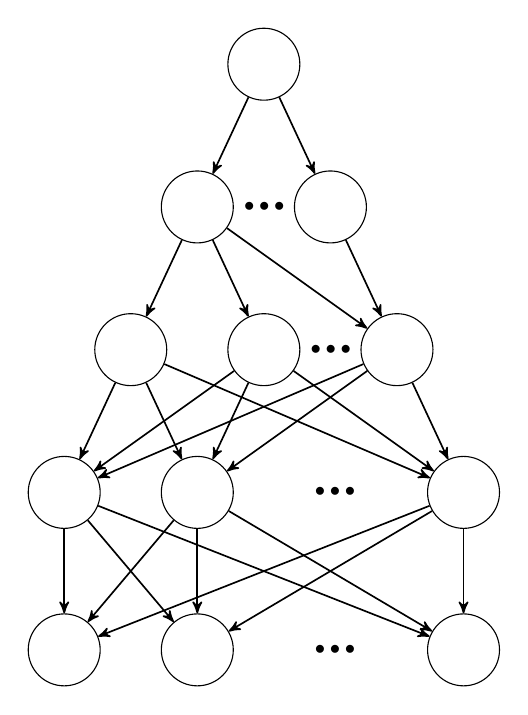
\begin{tikzpicture}
		[
		observed/.style={minimum size=15pt,circle,draw=blue!50,fill=blue!20},
		unobserved/.style={minimum size=26pt,circle,draw},
		post/.style={->,>=stealth',semithick},
		]
		% Layer 0
		\node (top) [unobserved] at (0,0) {};
		
		% Layer 1
		\node (l11) [unobserved] at ([shift=({245:2 cm})]top) {};
		\node (l12) [unobserved] at ([shift=({295:2 cm})]top) {};
		\node (l1_dots) [right of = l11, node distance=0.85cm] {\scalebox{0.75}{$\bullet\bullet\bullet$}};
		
		% Layer 2
		\node (l21) [unobserved] at ([shift=({245:2 cm})]l11) {};
		\node (l22) [unobserved] at ([shift=({295:2 cm})]l11) {};
		\node (l23) [unobserved] at ([shift=({295:2 cm})]l12) {};
		\node (l2_dots) [right of = l22, node distance=0.85cm] {\scalebox{0.75}{$\bullet\bullet\bullet$}};
		
		% Layer 3
		\node (l31) [unobserved] at ([shift=({245:2 cm})]l21) {};
		\node (l32) [unobserved] at ([shift=({295:2 cm})]l21) {};
		\node (l33) [unobserved] at ([shift=({295:2 cm})]l23) {};
		\node (l2_dots) [right of = l32, node distance=1.75cm] {\scalebox{0.75}{$\bullet\bullet\bullet$}};
		
		% Layer 4
		\node (l41) [unobserved] at ([shift=({270:2 cm})]l31) {};
		\node (l42) [unobserved] at ([shift=({270:2 cm})]l32) {};
		\node (l43) [unobserved] at ([shift=({270:2 cm})]l33) {};
		\node (l2_dots) [right of = l42, node distance=1.75cm] {\scalebox{0.75}{$\bullet\bullet\bullet$}};
		
		\path
		% Layer 0
		(top) edge [post] (l11)
		(top) edge [post] (l12)
		
		% Layer 1
		(l11) edge [post] (l21)
		(l11) edge [post] (l22)
		(l11) edge [post] (l23)
		(l12) edge [post] (l23)
		
		% Layer 2
		(l21) edge [post] (l31)
		(l21) edge [post] (l32)
		(l21) edge [post] (l33)
		(l22) edge [post] (l31)
		(l22) edge [post] (l32)
		(l22) edge [post] (l33)
		(l23) edge [post] (l31)
		(l23) edge [post] (l32)
		(l23) edge [post] (l33)
		
		% Layer 3
		(l31) edge [post] (l41)
		(l31) edge [post] (l42)
		(l31) edge [post] (l43)
		(l32) edge [post] (l41)
		(l32) edge [post] (l42)
		(l32) edge [post] (l43)
		(l33) edge [post] (l41)
		(l33) edge [post] (l42)
		(l33) edge [post] (l43)
		;
		
	\end{tikzpicture}}
	\caption{Illustration of the \gls{dag} structure for the five-level \gls{pam}.}	
	\label{fig:dag_structure}
\end{figure}




\subsubsection{Modification to Pachinko Allocation}\label{subsec:mod_pachinko}
Normally when working with topic modeling, one does not know which topics will be present in the document set before training the model.
However, the taxonomy metadata fields provide some general subject names of different levels of abstraction and some amount of documents attached to these subject names.
This provides a unique opportunity for using the existing taxonomies as higher-level topics.
Without modification, \gls{pam} will find topics with the same structure as our taxonomy, but the taxonomy values would be disregarded during training since it would generate new taxonomy sequences.
However, in our case, we have a partially observed taxonomy and we want to use the existing meta-information to estimate the topics quicker and more accurately.
Although, only ${\sim}25\%$ of the documents in our dataset have an observed taxonomy.
To account for this, we lock taxonomy for the words in the observed documents to be in the corresponding topics within the \gls{pam} \gls{dag} instead of continuously sampling them using Gibbs sampling.
This creates a constant context for the taxonomy topics, which the documents with unobserved taxonomies will be fitted around.

Some of the documents have multiple taxonomies.
For these documents, one of the taxonomies is chosen randomly for each word in the document. 


%
%\input{sections/method/preprocessing}
%\input{sections/method/method.tex}
%\input{sections/method/query_handling.tex}

%\section{Dataset}\label{sec:dataset}
Nordjyske is a Danish news agency that maintains multiple newspapers, radios, and other news sources throughout north Jutland, a region in Denmark.
They store their news articles in a non-public database, where each article contains multiple metadata fields which describe some aspect of the data, e.g., the author.
The dataset we use ranges from 2017 to 2019 and contains $248,385$ articles.

We perform some basic preprocessing to make the data more applicable for topic models.
Firstly, because the dataset includes articles from multiple cities and regions, duplicates do occur in the dataset.
These duplicates are removed, so only unique articles are kept.
After this, we filter out words that appear in less than 10 articles and words that appear in more than 10$\%$ of articles.
This is done to keep words that are used enough to find patterns in topics and to remove words that are similar to stop words.
Finally, after the words are filtered out, the empty documents are removed.
After preprocessing, the dataset contains $139,060$ articles that use a vocabulary of $69,192$ unique words.

The metadata fields that we are working with do have some problems that can be mitigated to a degree by preprocessing.
These problems are all related to some metadata values only being used in a few documents.
Since the metadata values are used to group documents together and find common topics and words within grouped documents, metadata values that group too few documents are not very relevant and are therefore combined or removed.

In the following sections, we describe each of the metadata fields which are analyzed.
Further details about the metadata labels can be seen in Appendix \autoref{sec:appendix_meta_data}.

\subsection{Author}
This field is for the author, who has written the article.
Each article only has a single author, so we do not account for multiple authors, whereas \citet{author_topic_2012} account for multiple authors.
This field is fully observed within the dataset, meaning that every article has an author.
Originally there were $227$ different authors within the dataset.
After combining authors that have written less than $14$ documents (${\sim}0.001\%$ of the total document set) into a 'misc' author of size $204$, $184$ authors remain.
%and they are almost evenly distributed in the number of articles they have written.

\subsection{Category}
% what it is?
The category field describes a variety of different aspects.
A proportion of the categories contains which specific newspaper they belong to, e.g., 'Aalborg-Newspaper'.
Another proportion of the category field describes the overall subject of the document, such as 'Culture' and 'Sports-newspaper'.
However, there are also nonsensical categories such as '53. Frederik', that do not seem to describe the subject of the document.
% stats
This field is fully observed within the dataset and there are originally $58$ different categories in the dataset.
However, while most of these categories cover a significant number of documents, some categories are only used by a few documents.
After combining all categories covering less than $140$ documents (${\sim}0.01\%$ of the total document set) into a single new 'misc' category of size $229$, $34$ categories remain.
The smallest category consists of $188$ documents, and for all categories, the median category size is $3022$.
\autoref{fig:category_box} shows an overview of the size of the categories after filtering.
The categories from the 3rd quartile and up do become much larger compared to the median, and there is an outlier category with $20,241$ documents.
These larger categories seem to be about topics that are written about often or categories that cover a specific newspaper.
All of the category labels can be seen in \autoref{tab:category_table} and the statistics in \autoref{tab:meta_prepro_stats}.
\todo[inline]{move 38 to 42 into appendix (starting with 'the smallest category'}

\subsection{Taxonomy}\label{sec:dataset_taxonomy}
The taxonomy field describes a hierarchical sequence of the topical or geographical subject of the articles.
Each sequence consists of several sub-taxonomies.
This field is only partially observed within the dataset, which means that ${\sim}25\%$ of the articles contain this field.
It is also possible for articles to contain multiple taxonomy sequences.
We observe some general patterns when traversing this field, which are:
\begin{itemize}
	\item PLACES/Country/Region/Town
	\item TOPICS/Sub-Topic/Subsub-topic
\end{itemize}
Examples of this field are:
\begin{itemize}
	\item PLACES/Danmark/Nordjylland/Aalborg/Lillevorde
	\item TOPICS/Religion/Christianity
\end{itemize}
About $80\%$ of the observed fields contain the 'PLACES' variable and $20\%$ use the 'TOPICS' variable.
There are also a few other top-level taxonomies; however, they are not as informative and are very rarely used.
Originally there were $1135$ different taxonomies; however, after removing taxonomies used by less than $14$ documents (${\sim}0.001\%$ of the total document set), $345$ remain.

%%\input{sections/Pipeline.tex}
\section{Evaluation}\label{sec:experiment}
In this section, we evaluate the topic models previously defined.
We also define the evaluation metrics, and how the hyperparameters for the models were chosen.
Lastly, the results of the evaluations are also shown.

\subsection{Models}\label{sec:experiment_models}
A list of different topic models is evaluated, each using different metadata from the dataset.
The main difference between the models is how they draw a specific topic for a word.
As detailed in \autoref{sec:plate_notation}, the main models used in this experiment are:
\begin{description}
	\item[\Acrlong{lda}] Standard \gls{lda}, which uses document-topic distributions.
	\item[Author-Topic Model]\cite{author_topic_2012} An \gls{lda} based model, which uses author-topic distributions.
	\item[Category-Topic Model] An \gls{lda} based model, which uses category-topic distributions.
	\item[Taxonomy-Topic Model] A \acrlong{pam} which uses hierarchical taxonomy information.
\end{description}

By extension of these models, combinations of the models are also evaluated.
As detailed in \autoref{sec:combinations}, these combinations are:
\begin{itemize}
	\item Author-Category
	\item Author-Taxonomy
	\item Category-Taxonomy
	\item Author-Category-Taxonomy
\end{itemize}
These model combinations should give insight into what a model learns when multiple metadata have influence on the topics chosen.

\subsection{Evaluation Metrics}\label{sec:experiment_metrics}
All models previously mentioned are evaluated on the following evaluation metrics.

The main metric used, in this experiment, is the topic coherence metric.
This metric indicates how semantically similar the top words within each topic are, and will be an indication of the quality of the topics of a topic model~\cite{topic_coherence_2015}.
There are many different methods for calculating topic coherence, but for this paper we will be using $C_v$ coherence.
$C_v$ is calculated using the following steps, as presented by~\citet{Syed2017coherence}:
\begin{enumerate}
	\item Topic-word segmentation into word set pairs
	\item Word and word pair probability calculation
	\item Word set confirmation measure
	\item Aggregation of confirmation measures
\end{enumerate}
The intuition is to calculate the degree of semantic similarity between highly probable words in a topic.
This intuition, and each step, is explained further in Appendix \autoref{app:topic_coherence}.

The second metric used in the experiment is perplexity.
Perplexity is used as a metric, to show how well a model can predict new test samples $w_d$.
But because perplexity is not specific to topic models, and by itself does not give an indication of how coherent topics are, it is mainly used as a secondary evaluation~\cite{tea_leaves}.
To calculate perplexity, we first need to compute the log-likelihood of $w_d$, which is done in:
\begin{equation}\label{eq:likelihood}
	\mathcal{L}(w_d) = \log p(w_d|\Phi) = \sum_{d} \log p(w_d|\Phi)
\end{equation}
\noindent where $\Phi$ is the topic-word matrix.
The perplexity measure is then calculated as follows:
\begin{equation}
	\emph{Perplexity}(w_d) = exp \{-\frac{\mathcal{L}(w_d)}{W}\}
\end{equation}
\noindent where W is the number of words \cite{de2008evaluating}.

Topic difference is another metric that is used to check the quality of the topic model.
It is based on the assumption that a good topic model will have little overlap between topics.
It is therefore not the best measure of the final quality of a topic model, but a low topic difference will indicate potential problems with a model.
\begin{equation}
	\emph{TopicDifference} = \frac{1}{K \cdot K} \sum_{i=1}^{K} \sum_{j=1}^{K} JS(\beta_{i},\beta_{j})
\end{equation}
\noindent where $JS$ is Jensen-Shannon distance, $K$ is the number of topics, and $\beta_{k}$ is the topic-word distribution for topic $k$.
If the total sum is not averaged out, this measure can also be used to indicate convergence of the model.

Finally, we also perform human evaluation of the topics generated.
\todo[inline]{How/if we do this is still to be discussed}

\subsection{Grid Search}\label{sec:experiment_gridsearch}
To find the optimal hyperparameter values for the models, we run a grid search.
In the grid search, different values of $K$, $\alpha$, and $\eta$ are tested to find the best performing model.
Specifically, we run two rounds of grid search.
In the first round, the number of topics $K$ we test are the values of $K_1$, as seen in \autoref{tab:gridsearch}, with randomly chosen $\alpha$ and $\eta$ values for each $K$ value.
This creates much fewer runs of the grid search to start with, and eliminates hyperparameter values that give clearly worse models.
In the second round, the number of topics $K$ we test are the values of $K_2$, with all combinations of $\alpha$ and $\eta$, except for those with values of $0.001$, since these models gave much worse scores.
The hyperparameter values that are tested, are shown in \autoref{tab:gridsearch}.

We only run the grid search on the standard \gls{lda} model, with the assumption that the number of topics that performs well for this model, also performs well for the metadata models, when the same dataset is used.
To evaluate the \gls{lda} models, we measure the topic coherence of a model after training it on the dataset for 50 epochs, and the hyperparameters of the model with the highest score are then used for the models in the rest of the experiment.

Based on the topic coherence of the model, we choose $K = 90$, $\alpha = 0.01$, and $\eta = 0.1$ as the hyperparameters for all models in the experiment.

\begin{table}[t]
	\centering
	\caption{Tested hyperparameter values for the grid search. $K_2$ are the $K$ values used for the grid search in conjunction with the bolded values in $\alpha$ and $\eta$.}
	\begin{tabular}{c|c}
		Parameter & Tested Values\\
		\midrule
		$K_1$ & 10, 20, 30, $\dots$, 100, 150\\
		$K_2$ & 50, 60 70, 80, 90, 100\\
		$\alpha$ & \textbf{0.1}, \textbf{0.01}, 0.001\\
		$\eta$ & \textbf{0.1}, \textbf{0.01}, 0.001\\
	\end{tabular}
	\label{tab:gridsearch}
\end{table}


\subsection{Results}\label{sec:results}

\begin{table}[h]
	\centering
	\caption{Results.}
	\begin{tabular}{l|c|c|c}
		Topic Model & Perplexity & \makecell{Topic \\ Coherence} & \makecell{Topic \\ Difference} \\
		\midrule
		\Acrlong{lda} & 6761.6 & 0.520 & 0.575 \\
		Author-Topic Model & 10991.5 & 0.335 & 0.615 \\
		Category-Topic Model & 11126.0 & 0.370 & 0.560 \\
		Taxonomy-Topic Model & - & 0.660 & 0.709 \\
	\end{tabular}
	\label{tab:metric_results}
\end{table}

From \autoref{tab:metric_results}, we can see that the Author and Category-Topic models are performing the worst, whereas the Taxonomy-Topic model is outperforming all other models.
However, the run time of the Taxonomy model is worse than the standard \gls{lda}.
It takes about 6-8 hours to compute 50 epochs for the \gls{lda} model, depending on the CPU. 
The Taxonomy model running a 5 layered \gls{pam} took 132 hours before completing the 50 epochs.
Extended analysis and other models are investigated in \autoref{subsec:app_exten_models} and \autoref{app:cat_auth_pachinko}.


%% - Body(50 \%)
%%	- Results 
%
%%	- Discussion
%%		- Main results
%%		- Other results
%%		- Error sources
\section{Model analysis}\label{sec:discussion}
In this section, we investigate the different models to see how each metadata affects the resulting topics.
Firstly, we want to investigate the most probable topic words within each model.
We have chosen an article arbitrarily from the dataset and visualized how the topics differ between the models. 
Before investigating the article, we define a specific color scheme for each model, which is seen in \autoref{tab:disc_color}.

In \autoref{fig:the_article}, we have highlighted the highest probable words within the three most probable topics in the article.
The article is about agriculture and how farmers opening their doors to the public. 
It also mentions a few different farms in the Northern part of Jutland and describes these in various ways.

\begin{table}
	\caption{Top 10 words of top 3 most occurring topics, within the article in \autoref{fig:the_article}, for each model used in \autoref{tab:disc_color}.}
	\label{tab:top_words_three_models}
	\begin{tabular}{c|p{0.8\columnwidth}}
		Topic & Top 10 words for \gls{lda} \\
		\midrule
		1 & sæby, a, direktør, frederikshavn, virksomheden, hans, medarbejdere, pedersen, firmaet, procent \\
		2 & omradet, boliger, natur, naturen, ligger, du, vand, dyr, a, skov \\
		3 & nielsen, arets, prisen, dansk, mors, jensen, løgstør, aars, vm, thy \\
	\end{tabular}
	\begin{tabular}{c|p{0.8\columnwidth}}
		\midrule
		Topic & Top 10 words for author-topic \\
		\midrule
		1 & du, procent, unge, børn, arige, hans, dansk, mig, thisted, mener\\
		2 & sine, skriver, mig, børn, seneste, land, dansk, kommuner, andersen, formand \\
		3 & set, glas, odense, vesthimmerland, leth, markedet, trump, ni, regionerne, prins\\
	\end{tabular}
	\begin{tabular}{c|p{0.8\columnwidth}}
		\midrule
		Topic & Top 10 words for category-topic \\
		\midrule
		1 & du, hans, børn, mig, thisted, procent, bedre, a, kr, maske \\
		2 & klar, haft, fem, hjørring, ham, nyt, formand, min, aften, sagen\\
		3 & du, min, gode, gamle, ad, henrik, eu, finde, sat, hobro\\
	\end{tabular}
	\begin{tabular}{c|p{0.8\columnwidth}}
		\midrule
		Topic & Top 10 words for taxonomy-topic \\
		\midrule
		1 & aab, jacob, kasper, rasmus, jakob, pedersen, andersen, friis, minut, allan \\
		2 & landbrug, landbruget, landmænd, vand, miljø, affald, bedre, natur, vandløb, fødevarer \\
		3 & virksomheden, millioner, a, direktør, procent, medarbejdere, selskabet, overskud, ansatte, virksomhed \\
	\end{tabular}
\end{table}

To compare these models, we take the top 200 words of the topic-word distributions within each model and mark them in the article.
We take 200 words since we want to see how intertwined the models are.
Since the Author and Category models do not have a document-topic distribution we can not look at the specific document, but instead, we have marked the words from the given category- and author-topic distribution for the documents category and author, to see what the difference in topics are.
\begin{table}[b]
	\centering
	\caption{Color scheme for each model.}
	\begin{tabular}{l|c}
		Topic Model & Color \\
		\midrule
		\Acrlong{lda} & \thiscolor{Goldenrod} \vspace*{2mm} \\
		Author-topic model & \thiscolor{Aquamarine} \vspace*{2mm} \\
		Category-topic model & \thiscolor{LimeGreen} \vspace*{2mm} \\
		Taxonomy-topic model & \thiscolor{Orchid} \vspace*{2mm} \\
		Word appearing in 3+ models & \thiscolor{Peach} \vspace*{2mm} \\
	\end{tabular}
	\label{tab:disc_color}
\end{table}
\newline
\begin{figure}[h]
	\begin{tcolorbox}[boxsep=5pt, top=0pt, bottom=0pt, left=0pt, right=0pt]
		\emph{
			kig på grise, køer og kyllinger10 \colorbox{Peach}{nordjyske} bedrifter åbner \mycolor{LimeGreen}{Aquamarine}{søndag} for stalddørene \mycolor{Orchid}{Goldenrod}{landbruget} åbner \mycolor{LimeGreen}{Aquamarine}{søndag} 16. \mycolor{Goldenrod}{Aquamarine}{september} ladeporte og stalddøre for offentligheden. 52 danske bedrifter er med i årets ”åbent \mycolor{Orchid}{Goldenrod}{landbrug}”. i det \colorbox{Peach}{nordjyske} kan man kigge forbi på 10 \colorbox{Peach}{forskellige} \mycolor{Orchid}{Goldenrod}{landbrug}. blandt de \colorbox{Peach}{nordjyske} deltagere er der \colorbox{Peach}{mulighed} for at få indsigt i både kvæg- og svinebedrifter, \colorbox{Peach}{ligesom} en producent af slagtekyllinger \colorbox{Aquamarine}{byder} velkommen. sidstnævnte kan opleves hos rokkedahl i farstrup. de er tre familier med i alt \colorbox{Peach}{seks} børn, der sammen driver rokkedahl \mycolor{Orchid}{Goldenrod}{landbrug} med slagtekyllinger og planteproduktion \colorbox{Peach}{samt} rokkedahl energi, som laver energioptimering. herudover har de \colorbox{Goldenrod}{eget} slagteri, hvor ca. 35 af deres i alt 65 \colorbox{Peach}{medarbejdere} arbejder. \colorbox{Goldenrod}{familien} rokkedahl har \colorbox{Peach}{arbejdet} med kyllinger siden 1963 og er tredje generation. i staldene og i de omkringliggende folde har de både fritgående og økologiske slagtekyllinger. velfærdskyllingerne går i flokke og har adgang til store folde. på årsbasis opdrætter rokkedahl \mycolor{Goldenrod}{Aquamarine}{otte} \colorbox{Peach}{millioner} kyllinger som enten slagtes på deres \colorbox{Goldenrod}{eget} slagteri eller sælges til eksterne slagterier. på de 1350 \mycolor{Orchid}{Goldenrod}{hektar} har de hvede, byg raps, havre, rug, ærter og hestebønner. det anvendes primært til foder til velfærdskyllingerne. de dyrker \colorbox{Peach}{jorden} primært økologisk og anvender halmen til opvarmning af staldene. de har varmevekslere på alle stalde for at minimere varmeforbruget og ammoniakudledningen til omgivelserne. britt og \colorbox{LimeGreen}{klaus} kristiansen på solbakken agri ved aabybro er \colorbox{Peach}{klar} til vise en stor, \colorbox{Peach}{dansk} mælkeproduktion frem. \colorbox{Goldenrod}{familien} tæller også de fire børn, maria på 18 år, daniel på 16 år, \colorbox{LimeGreen}{kamilla} og laura på 13 år, og de er sjette generation på gården, som de overtog i 2013. solbakken har 600 økologiske malkekøer, som tilsammen \colorbox{Peach}{giver} 17.000 liter mælk om dagen. den bliver hentet og kørt til et af arlas mejerier, hvor den bliver anvendt til økologiske mejeriprodukter. 575 \mycolor{Orchid}{Goldenrod}{hektar} \colorbox{Peach}{land} tilhører gården, og her producerer \colorbox{Goldenrod}{familien} foder til deres \colorbox{Peach}{dyr} \colorbox{Peach}{samt} andre fødevarer.  i himmerland kan man besøge sanne og \mycolor{LimeGreen}{Aquamarine}{ole} mathiasen, der driver nørregaard på braulstrupvej 9 i suldrup. her kan man se søer, smågrise og slagtesvin i staldene og \colorbox{Aquamarine}{høre} om \mycolor{Orchid}{Goldenrod}{produktion} af velfærdsgrise, se maskinerne, få smagsprøver fra \mycolor{Orchid}{Goldenrod}{danish} \colorbox{Goldenrod}{crown} og på \colorbox{Peach}{lokale} fødevarer, og \colorbox{Aquamarine}{høre} om biavl. for \colorbox{Aquamarine}{børnene} er der \colorbox{LimeGreen}{leg} i korncontainer og halm, pedaltraktorbane og ponytrækketure. der er kaffe og kagebord. åbent \mycolor{Orchid}{Goldenrod}{landbrug} foregår \mycolor{LimeGreen}{Aquamarine}{søndag} fra \colorbox{Peach}{klokken} 10 til 16. det er gratis at deltage. sidste år deltog 96.000 \mycolor{LimeGreen}{Aquamarine}{danskere} i åbent \mycolor{Orchid}{Goldenrod}{landbrug}.
		}
	\end{tcolorbox}
	\caption{An article chosen arbitrarily from our dataset where words within top 200 of the top 3 topics within each model are highlighted.}
	\label{fig:the_article}
\end{figure}

Overall, we see that there is a large amount of overlap between the models, which is interesting since the models use different metadata information to create the various topic distributions.
This indicates that the models share many of the top words, while also indicating a slight deviation between the models due to the metadata information.
The \gls{lda} model and the taxonomy model show words like "landbrug" (agriculture) and "produktion" (production), and "hektar" (acre) which is what the article is mostly about.
Author-topic specific words are not very present and are only showing three unique words: "byder", "hører", and "børnene".
This indicates that the author-topic model has trouble generalizing what the author of this article (Peter Tordrup Larsen) is writing about. 
This might be because he has written $5002$ articles in our dataset and generalizing that many articles is a challenge.
Another aspect of the author-topic model is that the authors writing these articles most likely do not write about just one subject, which explains why there are only three less important words marked here. 
The category-topic model only shows three unique words: "klaus", "kamilla", and "leg" (play).
These words are also very abstract and can be used in many different scenarios.

An interesting part of this analysis is the words appearing in three or more models.
Some notable words within this category are: "medarbejder" (co-worker), "arbejdet" (worked), "jorden" (earth), "land" (land), "nordjyske" (North Jutland), and "dyr" (animals).
These words are fairly representative of the content of the article.

A general pattern which can be seen in \autoref{fig:the_article} is that the \gls{lda} model and the taxonomy-topic model are marking many of the same words, where the taxonomy-topic model only occurs together with other models.
This makes sense because these two models have the best topic coherence in our results. 

There is also the possibility that choosing another random article would give completely different numbers of marked words per model because this highly depends on the article's author and category.
In Appendix \autoref{app:color_articles}, we investigate how the coloring applies to two other articles.

\begin{table}[t]
	\centering
	\caption{Top 10 author pairs based on the symmetric KL divergence between authors.}
	\begin{tabular}{r|c}
		Author pair & KL \\
		\midrule
		Lars Termansen (328) \& Mikkel Færgemann Viken (91) & 1.50 \\
		Morten Nis Klenø (17) \& Anne Helene Thomsen (606) & 1.72 \\
		Lars Termansen (328) \& Lars Christensen (1293) & 2.43 \\
		Esben Heine Pedersen (1689) \& Caspar Birk (71) & 2.47 \\
		Lars Christensen (1293) \& Poul Christoffersen (65) & 2.53 \\
		Lone Beck (92) \& Max Melgaard (587) & 2.74 \\
		HANNE Lindblad Jensen (27) \& Peter Tordrup Larsen (5002) & 2.94 \\
		Søren Kjær (95) \& Carl Chr. Madsen (785) & 2.98 \\
		Heidi Majgaard B. Pedersen (244) \& Lisbeth Helleskov (361) & 3.05 \\
		Lars Termansen (328) \& Morten Lind (413) & 3.16 \\
		\midrule
		Maximum & 34.51 \\
		Median & 24.20 \\
	\end{tabular}
	\label{tab:author_similarity}
\end{table}

\subsection{Author-topic model}\label{sec:discussion_author_topic}
Interesting observations can also be made specifically for the author-topic model.
The similarity of authors is a good example, which can be measured by taking the distance between their topic distributions.
In this model, the author-topic distribution defines the probabilities of topics being written by a specific author.
Then, just as \citet{author_topic_2012}, the similarity of authors can be found by calculating the symmetric Kullback-Leibler divergence:

\begin{equation} \label{eq:author_similarity}
	sKL(i,j) = \sum_{t=1}^{T}\left[\theta_{it}\, log \frac{\theta_{it}}{\theta_{jt}} + \theta_{jt}\, log \frac{\theta_{jt}}{\theta_{it}}\right]
\end{equation}
\todo{en sætning til at beskrive at theta i equation ovenfor er posterior probability from the gibbs sampler}
\noindent where $\theta_{it}$ is the probability of author $i$ having written about topic $t$, and the same for $\theta_{jt}$ with author $j$.

In the context of using these similarities for recommendation, knowing how similar authors are, gives the opportunity to recommend new authors to readers, while the articles are about similar topics.
In \autoref{tab:author_similarity}, the top 10 author pairs, based on this similarity measure, are shown.
A smaller KL value means the authors are more similar.
The number in parenthesis next to each author is the number of articles they have written in our dataset.

\begin{table}[h]
	\centering
	\caption{Top 10 author pairs based on the symmetric KL divergence between authors.}
	\begin{tabular}{r|c}
		Author pair & KL \\
		\midrule
		Lars Termansen (328) \& Mikkel Færgemann Viken (91) & 1.50 \\
		Morten Nis Klenø (17) \& Anne Helene Thomsen (606) & 1.72 \\
		Lars Termansen (328) \& Lars Christensen (1293) & 2.43 \\
		Esben Heine Pedersen (1689) \& Caspar Birk (71) & 2.47 \\
		Lars Christensen (1293) \& Poul Christoffersen (65) & 2.53 \\
		Lone Beck (92) \& Max Melgaard (587) & 2.74 \\
		HANNE Lindblad Jensen (27) \& Peter Tordrup Larsen (5002) & 2.94 \\
		Søren Kjær (95) \& Carl Chr. Madsen (785) & 2.98 \\
		Heidi Majgaard B. Pedersen (244) \& Lisbeth Helleskov (361) & 3.05 \\
		Lars Termansen (328) \& Morten Lind (413) & 3.16 \\
		\midrule
		Maximum & 34.51 \\
		Median & 24.20 \\
	\end{tabular}
	\label{tab:author_similarity}
\end{table}

In general, for these pairs, there does not seem to be a correlation between a high similarity and the categories of the articles they have written.
While one author in a pair might have mainly written for the sports category (Sport-avis) the other author might not have written for this category at all.
This can also be seen for categories that cover geographic locations, where one author might have written for Aalborg (Aalborg-avis) and the other author can have written for Thisted (Thisted-avis).

From sample documents written by the most similar author pair (Lars Termansen \& Mikkel Færgemann Viken), we find that both authors write a mix of regular news and sports articles.
Their high similarity could be due to the ratio between news and sports news for both authors being similar, and possibly also because of the types of news they write about.
Another interesting observation is that, for the second most similar author pair (Morten Nis Klenø \& Anne Helene Thomsen) the difference in the number of articles written is significant.
Here Morten Nis Klenø has written just 17 articles while Anne Helene Thomsen has written 606 articles.
This suggests that some part of why these authors' similarity is high, simply depends on the types of news the authors have written, no matter the amount.

It is also worth noting that while authors that write scientific papers usually write in just a few subject areas, the scientific area they work in, this is not necessarily the case for news article authors.
In our dataset, this can be seen in the fact that the authors have written for 7.86 categories on average, with 7 categories as the median.
This can make it more difficult for the author-topic model to find patterns in what the authors write about, especially since each category can cover multiple topics.

A random selection of authors from the dataset and the top words from their most probable topic can be seen in \autoref{tab:author_top_words}.

\begin{table*}[h]
	\centering
	\caption{Selection of authors/categories and the top 10 words from their most probable topic.}
	\begin{tabular}{c|c|c|c|c|c|c}
		\toprule
		\multicolumn{7}{c}{Authors} \\
		\midrule
		Birgitte Bové & Kirsten Østergaard & Pauline Bülow & Karen Marie Foldbjerg & Claus T. Kræmmergård & Hanne Lindblad Jensen & Ole Jensen \\
		\midrule
		Topic 41 & Topic 50 & Topic 3 & Topic 13 & Topic 88 & Topic 2 & Topic 50 \\
		\midrule
		\makecell{millioner \\ eu \\ hans \\ større \\ bedre \\ formand \\ kr \\ nordjyske \\ taget \\ skriver} & \makecell{du \\ thisted \\ unge \\ mig \\ børn \\ procent \\ hans \\ hver \\ penge \\ hjørring} & \makecell{procent \\ bag \\ rigtig \\ lave \\ dansk \\ formand \\ gode \\ klar \\ svært \\ plads} & \makecell{du \\ sine \\ formand \\ seneste \\ jensen \\ hvert \\ nyt \\ hvordan \\ finde \\ kommunen} & \makecell{du \\ procent \\ unge \\ børn \\ arige \\ hans \\ dansk \\ mig \\ thisted \\ mener} & \makecell{du \\ thisted \\ procent \\ mig \\ børn \\ hans \\ unge \\ dansk \\ mener \\ a} & \makecell{du \\ thisted \\ unge \\ mig \\ børn \\ procent \\ hans \\ hver \\ penge \\ hjørring} \\
		\midrule
		\multicolumn{7}{c}{Categories} \\
		\midrule
		Frieord & Bo Godt & WEEKEND & Mariagerfjord-avis & Aalborg-avis & Navne & Sport-avis \\
		\midrule
		Topic 37 & Topic 7 & Topic 31 & Topic 39 & Topic 63 & Topic 14 & Topic 39 \\
		\midrule
		\makecell{du \\ thisted \\ mig \\ hans \\ procent \\ børn \\ a \\ kr \\ arige \\ unge} & \makecell{du \\ børn \\ mig \\ hans \\ unge \\ procent \\ mener \\ politiet \\ hvordan \\ thisted} & \makecell{du \\ hans \\ børn \\ mig \\ thisted \\ procent \\ bedre \\ a \\ kr \\ maske} & \makecell{du \\ thisted \\ dansk \\ unge \\ mig \\ børn \\ a \\ hans \\ procent \\ arbejde} & \makecell{børn \\ hver \\ thy \\ rigtig \\ millioner \\ synes \\ mennesker \\ ham \\ mand \\ dansk} & \makecell{hver \\ haft \\ bedre \\ ham \\ thy \\ mener \\ hans \\ mig \\ nordjylland \\ plads} & \makecell{du \\ thisted \\ dansk \\ unge \\ mig \\ børn \\ a \\ hans \\ procent \\ arbejde} \\
		\bottomrule
	\end{tabular}
	\label{tab:author_top_words}
\end{table*}

\subsection{Category-topic model}\label{sec:discussion_category_topic} 
Specific observations for the category-topic model can also be made.
As with the author-topic model, the similarity between pairs of categories can be calculated.
Because topic distributions are generated for each category, category similarity can also be calculated using \autoref{eq:author_similarity} where $i$ and $j$ are categories instead of authors.
In \autoref{tab:category_similarity}, the top 10 category pairs, based on symmetric KL divergence, are shown.

The second most similar pair, 'Friii' and 'Debat', is interesting to look at since 'Friii' does not seem to have a theme in the articles written, articles with the 'Debat' (debate) category seem to mostly cover themes that can bring differing opinions and articles with interviews.
This indicates that the model does not find these deeper thematic differences in articles or that it finds other patterns that are difficult to see.

It is also interesting that the 'misc' category is seen twice in the top 10 ranking even though it is made up of many smaller categories with no connection to each other.
Though, it is not surprising that this thematically mixed category is quite similar to 'Friii' and 'Debat', which are more thematically wide categories.

It is also clear that some of the topics that the model has learned fit well with how some categories are used in the dataset.
For example, the 4th ranking pair 'Sport-avis' and 'Morsø Sport' are clearly correlated by their category names covering sports news and the similarity of the topic distributions learned for both categories indicates that the model has learned these sports topics correctly.

Finally, it is worth noting that there are no category pairs, where both categories are based on geographic locations, in the top 10 pairs.
This may indicate that each city or municipality in Denmark does have some differences in which topics are written about in general.

A random selection of categories from the dataset and the top words from their most probable topic can be seen in \autoref{tab:author_top_words}.

This knowledge about categories can support recommendation in multiple ways.
An example is, that while news sites often have the possibility to filter articles based on categories, knowing which categories are similar gives further opportunities for recommending related or similar articles.

\begin{table*}[t]
	\centering
	\caption{Top 10 words of selected topics from our taxonomy-topic model. Labels have been manually added to the topics to increase readability.}
	\label{tab:pachinko_selected_topics}
	\begin{tabular}{c | c | c}
		Topic & Label & Top 10 words \\
		\hline
		8 & politics & venstre, valg, valget, partiet, partier, parti, stemmer, mette, politik, regering \\
		9 & money & procent, viser, tal, antallet, milliarder, pct, seneste, penge, millioner, indland \\
		19 & filler & mig, maske, du, folk, synes, ting, faktisk, nogen, altid, tror \\
		21 & university & unge, uddannelse, studerende, gymnasium, elever, uddannelser, universitet, procent, uddannelsen, nordjylland \\
		41 & academic research & universitet, professor, forskere, forskning, forskerne, viser, verden, institut, procent, aarhus \\
		42 & filler & mig, min, mit, ham, aldrig, gik, lille, maske, mine, altid \\
		45 & wildlife & dyr, naturen, natur, ulve, fugle, ulven, arter, dyrene, vilde, ulv \\
		47 & church & kirke, kirken, sognepræst, præst, søndag, koret, gudstjeneste, aften, kor, organist \\
		59 & music concerts & musik, koncert, sange, spiller, koncerter, band, koncerten, festival, musikken, publikum \\
		60 & buisness & virksomheden, millioner, a, direktør, procent, medarbejdere, selskabet, overskud, ansatte, virksomhed \\
		69 & primary school & elever, unge, skole, eleverne, skolen, skoler, klasse, børn, folkeskolen, lærere \\
		74 & elder care & ældre, borgere, kommunen, millioner, penge, nordjylland, plejehjem, borgerne, kommunens, budget \\
		75 & filler & du, din, dig, dit, altsa, dine, maske, nemlig, bruge, hvordan \\
		79 & filler & mig, min, hendes, hende, rigtig, arige, altid, arbejde, mor, mine \\
		86 & sports & handbold, mors, thy, hold, kamp, sæson, kampe, kampen, point, holdet \\
	\end{tabular}
\end{table*}


\begin{table*}[t]
	\centering
	\caption{IDs of the 5 most occurring fourth layer topics for each third layer topic from the taxonomy-topic model. See \autoref{tab:pachinko_selected_topics} and Appendix \autoref{tab:pachinko_topics} for the most occurring words for each ID.}
	\label{tab:pachinko_mid_topics}
	\begin{tabular}{c | c | c | c | c | c}
		Taxonomy Name & Top 5 Topic IDs & Taxonomy Name & Top 5 Topic IDs & Taxonomy Name & Top 5 Topic IDs \\ \hline
		Danmark & 8, 42, 82, 59, 79 & Udland & 42, 79, 59, 8, 32 & Kultur & 9, 42, 79, 19, 8 \\
		Landbrug & 42, 79, 8, 9, 19 & Kriminalitet & 42, 75, 60, 8, 86 & Socialstof & 42, 9, 79, 86, 8 \\
		Arbejdsmarked & 42, 79, 59, 8, 9 & Økonomi & 79, 75, 74, 42, 9 & Sundhed & 8, 32, 42, 9, 19 \\
		Politik & 42, 75, 9, 19, 74 & Musik & 75, 42, 59, 11, 79 & Sport & 42, 75, 8, 59, 52 \\
		Bolig & 75, 42, 86, 79, 8 & Videnskab & 42, 8, 52, 79, 19 & Trafik & 42, 74, 8, 52, 32 \\
		Erhverv & 42, 8, 59, 32, 79 & Uddannelse & 42, 9, 75, 32, 74 & Energi & 42, 8, 79, 19, 86 \\
		Ulykker & 42, 75, 9, 79, 32 & Fritid & 42, 8, 75, 82, 79 & Socialt & 42, 75, 79, 59, 9 \\
		Dyr & 86, 42, 79, 52, 9 & Natur & 42, 52, 9, 32, 79 & Miljø & 8, 42, 75, 52, 59 \\
		Familie & 79, 8, 42, 59, 32 & Politi & 42, 75, 79, 8, 59 & Byggeri & 75, 42, 79, 77, 59 \\
		Etik & 79, 42, 8, 86, 74 & Religion & 42, 79, 8, 59, 32 & Kommunalvalg & 42, 8, 75, 79, 32 \\
		Nordjyske Plus & 42, 86, 9, 79, 74 & DF & 42, 8, 59, 52, 19 & & \\
	\end{tabular}
\end{table*}
\subsection{Taxonomy-topic model}\label{sec:taxonomy_analysis}\vejleder{titel \# topics?}
Finally, we also want to analyze the taxonomy-topic model, especially since this model has the highest topic coherence out of all the tested models.
\autoref{tab:pachinko_topics} in the appendix shows the final lowest level topics of the taxonomy-topic model.
Note that while most of the topics are semantically coherent, there are some topics (e.g., topic 19 and 42) that consist entirely of words that provide little context or semantic meaning.
This indicates that the model has learned to group words that do not belong to any good topics.
This is a good feature that allows the model to apply an extra layer of preprocessing, automatically filtering away irrelevant words into topics.
This feature is also seen in some other topic models, such as in the hierarchical \gls{lda} (hLDA) by \citet{hLDA2004} and the embedded topic model (ETM) by \citet{dieng2020topic}, but the \gls{lda} does not seem to have this feature.

Since this model deals with more topic distributions than the other models, it is worth checking whether it also converges within the first 50 epochs, as with \gls{lda}.
This does seem to be the case, as indicated by \autoref{fig:pachinko_train}.
Here it can be seen that the topic coherence curve has flattened significantly, and thus additional epochs will have diminishing returns.\vejleder{what about LL?}

\begin{figure}
	\centering
	\includegraphics[width= \linewidth]{figures/pachinko_training.PNG}
	\caption{Topic coherence during training of the taxonomy-topic model.}
	\label{fig:pachinko_train}
\end{figure}

\autoref{tab:pachinko_mid_topics} gives an overview of how the taxonomy topics in the third layer of the taxonomy-topic model, are connected to the fourth layer topics that were generated by the model.
Some of these connections make a lot of sense, such as the 'Økonomi' (Economy) topic which has the three filler\vejleder{explain filler} topics: 79, 75, and 42, which consists of words with little semantic value, and two topics which are about money: 74 and 9.
However not all the connections\vejleder{the connections make er understreget} make as much sense as these. 
For example, the 'Kriminalitet' (Crime) topic has two filler topics: 42 and 75, one topic about economy: 60, one topic about politics: 8, and one topic about sports: 86.
See \autoref{tab:pachinko_topics}, for more details on the top words within each of these topics.
\vejleder{uddyb gerne}
Having the layered structure of the \gls{pam} gives many possibilities for recommending new articles to readers.
There is the possibility of exploring the similarity of taxonomies at the same layer and using this to recommend new articles with similar subjects.
For example, if an article is about 'Miljø' (environment) similar taxonomies might be 'Natur' (nature) and possibly 'Etik' (ethics), 'Trafik' (traffic), and 'Energi' (energy).

\begin{table*}[h]
	\centering
	\caption{IDs of the top 5 most occurring fourth layer topics for each third layer topic from the pachinko model. See \autoref{tab:pachinko_topics} for the most occurring words for each ID.}
	\label{tab:pachinko_mid_topics}
	\begin{tabular}{c | c | c | c | c | c}
		Taxonomy Name & Top 5 Topic IDs & Taxonomy Name & Top 5 Topic IDs & Taxonomy Name & Top 5 Topic IDs \\ \hline
		Danmark & 8, 42, 82, 59, 79 & Udland & 42, 79, 59, 8, 32 & Kultur & 9, 42, 79, 19, 8 \\
		Landbrug & 42, 79, 8, 9, 19 & Kriminalitet & 42, 75, 60, 8, 86 & Socialstof & 42, 9, 79, 86, 8 \\
		Arbejdsmarked & 42, 79, 59, 8, 9 & Økonomi & 79, 75, 74, 42, 9 & Sundhed & 8, 32, 42, 9, 19 \\
		Politik & 42, 75, 9, 19, 74 & Musik & 75, 42, 59, 11, 79 & Sport & 42, 75, 8, 59, 52 \\
		Bolig & 75, 42, 86, 79, 8 & Videnskab & 42, 8, 52, 79, 19 & Trafik & 42, 74, 8, 52, 32 \\
		Erhverv & 42, 8, 59, 32, 79 & Uddannelse & 42, 9, 75, 32, 74 & Energi & 42, 8, 79, 19, 86 \\
		Ulykker & 42, 75, 9, 79, 32 & Fritid & 42, 8, 75, 82, 79 & Socialt & 42, 75, 79, 59, 9 \\
		Dyr & 86, 42, 79, 52, 9 & Natur & 42, 52, 9, 32, 79 & Miljø & 8, 42, 75, 52, 59 \\
		Familie & 79, 8, 42, 59, 32 & Politi & 42, 75, 79, 8, 59 & Byggeri & 75, 42, 79, 77, 59 \\
		Etik & 79, 42, 8, 86, 74 & Religion & 42, 79, 8, 59, 32 & Kommunalvalg & 42, 8, 75, 79, 32 \\
		Nordjyske Plus & 42, 86, 9, 79, 74 & DF & 42, 8, 59, 52, 19 & & \\
	\end{tabular}
\end{table*}


%
%
%% - Conclusion (5 \%)
%%	- (Possible) Future work
\section{Conclusion}\label{sec:conclusion}
We explore possibilities of incorporating meta-data into existing topic models, such as \gls{lda} and \gls{pam}.
We evaluate three different metadata, Author, Category, and Taxonomy, each of which represent the data in a different way.
From the topic coherence results, shown in \autoref{tab:metric_results}, the \gls{pam} model using the Taxonomy meta data gets the best results.
The Author and Category models are the worst performing, where the topic coherence is much lower than the other models.
We want to answer the problem statement, which we stated in \autoref{sec:introduction}:

\begin{itemize}
	\item \textit{How does including metadata within the \gls{lda} model impact the resulting topics?}
	\item \textit{What possible problems can these models help alleviate at Nordjyske?}
\end{itemize}

Incorporating metadata into a topic model can be done various ways, and we incorporate them in multiple ways.
The \gls{lda} model is used as a baseline, which indicates whether incorporating metadata can improve the topic quality of our topic models.
Based on our analysis, we see that only using the metadata for topic assignment within \gls{lda}, can hurt the topic quality, which is how Author-Topic and Category-Topic is run.

We use the \gls{pam} to incorporate a hierarchical structured metadata called Taxonomy, where we use a novel locking mechanism to lock the observed metadata's topic into place.
Using this technique and model, we are able to get better topic quality and words within \gls{pam} compared to the \gls{lda}.
However, the run time for the algorithm is quite slower than the \gls{lda}.





\section{Future Work}\label{sec:future_work}
Due to the promising results provided by the modified pachinko model, investigating this model further might be beneficial to incorporating meta-data into topic models.
However, testing these model on multiple datasets, needed to be accounted for, since the generalizability of these models is not explored within this paper.
Using word embedding to further improve the performance of models can also be viewed as the next step for this project, since a wide number of papers are using this technique to improve topic modeling.


Using these models at Nordjyske, would also be very interesting to see, how we could incorporate them into a existing IT infrastructure.
The next step in that process, would be to investigate which part of their infrastructure could benefit from the use of topic modeling, whether it is recommendation or automatic tagging of articles. 
We have written about a few potential use cases for our project in \ref{sec:appendix_applications} in the Appendix. 

%
%\input{sections/Acknowledgements}

% - References (10 \%)
% 	- Acknowledgments
%	- Bibliography
\vejleder[inline]{Expand the citation list!!}
\bibliography{paper}

%Appendixes, if needed, appear before the acknowledgment.
\glsresetall
\onecolumn
\appendix
% Intro
In the main paper, we initialize and describe our problem with a focus on results. \vejleder{kun et niveau?}
Within this appendix, we are expanding on many aspects of the aforementioned paper and describing new experiments that have been made.

This includes:
\begin{itemize}
	\item Overview
	\begin{itemize}
		\item A brief explanation of the process of training and evaluating our models.
	\end{itemize}
	\item Expanding on the paper
	\begin{itemize}
		\item The metadata is shown in tables for all three metadata types, and observations about the metadata labels are described.
		\item We explain the purpose and mathematical ideas behind the evaluation metrics we use in the paper.
		\item Our grid search process is described further on how we chose our hyperparameters.
		\item More articles are highlighted the same way as in \autoref{sec:discussion} and observations are made.
	\end{itemize}
	\item Code
	\begin{itemize}
		\item An experiment using a stemmed dataset is described, and the results are observed.
		\item We describe the probabilistic programming language Pyro which we explored before choosing to work with Gibbs sampling.
		\item The code for the Gibbs sampler is explained and how the \gls{pam} differs from the standard Gibbs Sampler is described. 
		\item Our testing of a parallel Gibbs sampler is also described.
	\end{itemize}
	\item Expanded model experiments
	\begin{itemize}
		\item We go into detail how we explored using author and category metadata in the \gls{pam} and what results were achieved.
		\item We also explored a model combining the author-topic and category-topic models into one model with two topic distribution. This model is also analyzed.
		\item Further model combinations we explored, were models that combine the standard \gls{lda} with our author and category metadata models.
	\end{itemize}
	\item Applications
	\begin{itemize}
		\item We explore the application possibilities of our project and propose various applications which could be implemented at Nordjyske.
	\end{itemize}
\end{itemize}


% Overview
\subsection{Overview}\label{sec:overview}
This section describes the steps of our method on an abstract level.
\autoref{fig:process_figure} visualizes these steps as a flowchart.
The method takes a corpus as an input and produces evaluation results as output.
Each step of the method is described in more detail in the paper.

\subsubsection*{Step 1: Preprocessing phase}
In this step, we apply different preprocessing methods to simplify the dataset and remove redundant information.
Details of this phase are given in \autoref{sec:dataset}.
After finishing this phase, we are left with $139,060$ articles and $69,192$ unique words to form the corpus, which is used in the following steps.

\subsubsection*{Step 2: Training topic models}
In this step, we train the standard \gls{lda} model, and the category, author, and taxonomy metadata models, on the corpus.
The standard \gls{lda} model and the metadata models are described in \autoref{sec:plate_notation}.
The models are trained based on topic coherence, and after the training process, the models are evaluated further.

\subsubsection*{Step 3: Evaluation of topic models}
In this step, we set up an evaluation for the topic models trained in the previous step.
The primary evaluation metric chosen for the experiment is topic coherence, and this is calculated for all of the models.
We also analyze the generated topics to get a deeper understanding of what the models learn.
The evaluation and results are presented in \autoref{sec:experiment} and are analyzed and discussed in \autoref{sec:discussion}.

\tikzstyle{process} = [rectangle, rounded corners, minimum width=2cm, minimum height=1cm,text centered, draw=black, fill=gray!50]
\tikzstyle{decision} = [diamond, minimum width=2cm, minimum height=1cm, text centered, draw=black, fill=green!30]

% one line
%\begin{figure}[ht]
%    \centering
%    \begin{tikzpicture}[node distance=2cm]
%    %\draw[step=1cm,gray,very thin] (-8,-8) grid (8,8);
%	\node (Dataset) [process] {(Input) Nordjyske Dataset};
%	\node (Cleaning)[process, below of=Dataset] {(1) Preprocessing Phase};
%	\node (Training) [process, below of=Cleaning] {(2)Train IR Methods};
%	\node (Query) [process, below of=Training] {(3) Query Generation};
%	\node (Evaluate) [process, below of=Query] {(4) Evaluate Models};
%	\node (Result) [process, below of=Evaluate] {(Output) Results};
%	\draw [->, very thick] (Dataset) edge (Cleaning); 
%	\draw [->, very thick] (Cleaning) edge (Training);
%	\draw [->, very thick] (Training) edge (Query);
%	\draw [->, very thick] (Query) edge (Evaluate);
%	\draw [->, very thick] (Evaluate) edge (Result);
%\end{tikzpicture}
%	\caption{The method visualized as a flowchart, where a dataset consisting of articles is processed into a list of ranked results.}
%    \label{fig:process_figure}
%\end{figure}

\begin{figure}[ht]
	\centering
	\begin{tikzpicture}[node distance=6em]
	%\draw[step=1cm,gray,very thin] (-8,-8) grid (8,8);
	\node (Dataset) [process, label=left:{Input}] {Nordjyske Dataset};
	\node (Cleaning)[process, below of=Dataset, label=left:{Step 1}] {Preprocessing};
	\node (Training) [process, below of=Cleaning, label=left:{Step 2}] {Train Topic Models};
	%\node (Query) [process, below of=Dataset, label=Step 3, yshift=2.5cm] {Query Generation};
	\node (Evaluate) [process, below of=Training, label=left:{Step 3}] {Evaluate Topic Models};
	\node (Result) [process, below of=Evaluate, label=left:{Output}] {Results};
	\draw [->, very thick] (Dataset) edge (Cleaning); 
	\draw [->, very thick] (Cleaning) edge (Training);
	\draw[->, very thick] (Training) edge (Evaluate);
	%\draw [->, very thick] (Query) edge (Evaluate);
	\draw [->, very thick] (Evaluate) edge (Result);
	\end{tikzpicture}
	\caption{The method visualized as a flowchart, where a dataset consisting of articles is processed into a list of evaluation results.}
	\label{fig:process_figure}
\end{figure}

\subsection{Metadata labels}\label{sec:appendix_meta_data}
In this section, the different types of metadata used in our evaluations will be explored. 
Here the focus will be on observations related to the labels of the metadata.

\subsection{Metadata labels}\label{sec:appendix_meta_data}

\subsubsection{Category}\label{subsec:appendix_category}

Here are the $58$ different categories, which make up all the category labels present within the dataset.
Categories with fewer than 139 documents ($0.1$ of the number of documents) are removed as part of preprocessing and replaced with a single miscellaneous category 'misc'.
This reduces the number of categories to $34$, while only replacing 292 documents to have the 'misc' category.
This preprocessing also makes the size of the remaining categories much more evenly distributed, as can be seen in \autoref{fig:category_hist}.

\begin{figure*}[ht]
	\centering
	\begin{subfigure}{0.45\textwidth}
		\centering
		\includegraphics[width=\linewidth]{figures/category_hist2_before.png}
		\caption{Before preprocessing}
		\label{fig:category_hist_before}
	\end{subfigure}
	\begin{subfigure}{0.45\textwidth}
		\centering
		\includegraphics[width=\linewidth]{figures/category_hist2_140.png}
		\caption{After preprocessing}
		\label{fig:category_hist_after}
	\end{subfigure}
	\caption{Histogram over the number of categories for different number of documents, before and after preprocessing.
	Categories on the x-axis are grouped into 50 buckets.}
	\label{fig:category_hist}
\end{figure*}

As mentioned in \autoref{sec:dataset}, some nonsensical categories are worth mentioning.
Specifically, the categories '26. Frederik' and '53. Frederik' do not from their names indicate what they cover, since Frederik is simply a normal Danish name.
Since they are not filtered into the 'misc' category during preprocessing, it is worth looking into what documents have these categories.

By looking at a random selection of documents from these categories, there is no clear pattern to be found.
The topics, within these categories, can be about anything from sports to news from anywhere around the world or locally in Denmark.
The articles from '26. Frederik' appear all years in our dataset, while the articles for '53. Frederik' seem to be just from 2019, the last year in our dataset, but evenly distributed over the whole year.
Curiously enough, most of the documents from these categories seem to be written by Anders Kjærgaard, with only a few other authors.
For '26. Frederik' there are just 5 unique authors: Carsten Tolbøll, Emil Abkjær Kristensen, Morten Kyndby Holm, Jens Fogh-Andersen, and Anders Kjærgaard.
For '53. Frederik' there are just 4 unique authors: Klaus Færch Gjerulff, Morten Kyndby Holm, Jens Fogh-Andersen, and Anders Kjærgaard.
This shows that Morten Kyndby Holm, Jens Fogh-Andersen, and Anders Kjærgaard have written for both categories.

From the exploration of these two categories, we can not say with certainty why these categories exist, or why multiple authors have chosen to write for these categories.
We continue to use these categories in our experiment, for the possibility of making other observations through the topic models.

\begin{table*}[h]
	\centering
	\begin{tabular}{l|c|l|c|l|c|l|c}
		Category            & Number & Category        & Number & Category                       & Number & Category                    & Number \\
		\toprule
		Fælles              & 20204  & Navne           &  3749  & Kram                           &  244   & \textbf{Østvendsyssel Avis} &   4    \\
		Thisted-avis        & 11473  & Kultur          &  3012  & 53. Frederik                   &  203   & \textbf{DF Motor Biler}     &   3    \\
		Sport-avis          & 10941  & Morsø Sport     &  2350  & Feature                        &  188   & \textbf{Nyhedsmotoren-net}  &   3    \\
		Debat               & 10075  & Friii           &  2333  & \textbf{Aalborg:nu}            &   73   & \textbf{Plus Publicering}   &   3    \\
		Udland-avis         &  8855  & Bagside         &  1933  & \textbf{Erhvervsnavne}         &   39   & \textbf{RB}                 &   3    \\
		Erhverv-avis        &  7356  & MitLiv          &  1519  & \textbf{Newspack}              &   35   & \textbf{Sport-net}          &   3    \\
		Mariagerfjord-avis  &  7241  & WEEKEND         &  1493  & \textbf{DF Søfart}             &   32   & \textbf{Thisted-net}        &   3    \\
		Morsø-avis          &  5959  & Bo Godt         &  1447  & \textbf{Morsø Ugeavis}         &   27   & \textbf{Hanbo-bladet}       &   2    \\
		Aalborg-avis        &  5544  & Nordjyske Biler &  1400  & \textbf{DF Licitation Byggeri} &   14   & \textbf{Brugermappe}        &   1    \\
		Vesthimmerland-avis &  5131  & Morsø Debat     &  1375  & \textbf{Biler}                 &   13   & \textbf{Brønderslev-net}    &   1    \\
		Rebild-avis         &  4415  & Frieord         &  1341  & \textbf{Samfund}               &   9    & \textbf{Lokalavisen}        &   1    \\
		Frederikshavn-avis  &  4325  & Indsigt         &  984   & \textbf{Nordjyske Plus}        &   6    & \textbf{Mariagerfjord-net}  &   1    \\
		Hjørring-avis       &  4235  & Thisted sport   &  698   & \textbf{Oplandsavisen}         &   6    & \textbf{Morsø-net}          &   1    \\
		Brønderslev-avis    &  3857  & Perspektiv      &  613   & \textbf{INFOMAKER PRINT}       &   5    &                             &        \\
		Jammerbugt-avis     &  3791  & 26. Frederik    &  484   & \textbf{DF Licitation Diverse} &   4    &                             &        \\
		\bottomrule
	\end{tabular}
	\caption{Amount of documents for each of the 58 categories within the Nordjyske dataset from 2017 to 2019.
		The highlighted categories are filtered and combined during preprocessing.}
	\label{tab:category_table}
\end{table*}
\todo[inline]{mark categories that are preprocessed away}


\subsubsection{Author}\label{subsec:appendix_author}
Unlike with Categories, the Author metadata field does not have a natural cut-off point, with a good amount of values in a specific lower range, followed by more evenly distributed numbers.
Instead, the vast majority of the values fall in a lower range, meaning that setting too high a cut-off point, will result in removing a large portion of the data.
We instead choose a lower cut-off point, keeping most of the authors, except the ones that contained so few documents, that finding common topics would be inefficient.
Authors, who have written less than $14$ documents ($0.01\%$ of the number of documents), are removed as part of preprocessing.
This removes $43$ out of $227$ authors, combining them into a single 'misc' author.
A total of $204$ documents are assigned to the 'misc' author.
\todo[inline]{figure out whether to use boxplots or histograms, and ref them.}

\begin{figure*}[ht]
	\centering
	\begin{subfigure}{0.45\textwidth}
		\centering
		\includegraphics[width=\linewidth]{figures/author_hist2_before.png}
		\caption{Before preprocessing}
		\label{fig:author_hist_before}
	\end{subfigure}
	\begin{subfigure}{0.45\textwidth}
		\centering
		\includegraphics[width=\linewidth]{figures/author_hist2_14.png}
		\caption{After preprocessing}
		\label{fig:auhtor_hist_after}
	\end{subfigure}
	\caption{Histogram over amount authors who have written certain number of documents, before and after preprocessing.
	Authors on the x-axis are grouped into 50 buckets.}
	\label{fig:author_hist}
\end{figure*}

\begin{figure*}[ht]
	\centering
	\begin{subfigure}{0.45\textwidth}
		\centering
		\includegraphics[width=\linewidth]{figures/author_box_before.png}
		\caption{Before preprocessing}
		\label{fig:author_box_before}
	\end{subfigure}
	\begin{subfigure}{0.45\textwidth}
		\centering
		\includegraphics[width=\linewidth]{figures/author_box_14.png}
		\caption{After preprocessing}
		\label{fig:auhtor_box_after}
	\end{subfigure}
	\caption{Boxplot over the amount of documents written by authors.}
	\label{fig:author_box}
\end{figure*}

\subsubsection{Taxonomy}\label{subsec:appendix_taxonomy}
Taxonomy is fundamentally different from the other metadata fields, in this paper.
It is not fully observed with only roughly $25\%$ of documents having a taxonomy field.
It is hierarchical, with each taxonomy containing a sequence of sub-taxonomies, such as: 'STEDER/Danmark/Nordjylland/Aalborg'.
It is also possible for each document to have multiple taxonomy sequences.
We remove any sub-taxonomy that is used in less than $4$ taxonomy sequences.
Out of $1135$ sub-taxonomies, $522$ are removed during this preprocessing.
\todo[inline]{describe layer sizes of taxonomy tree}

\begin{table}
	\begin{tabular}{l | c | c | c | c | c}
		Metadata & Min & Max & Mean & Median & Std. \\
		\hline
		Author & 1 & 9893 & 612.6 & 191 & 1219.7 \\
		Author (preprocessed) & 15 & 9893 & 751.7 & 323 & 1311.9 \\
		Category & 1 & 20204 & 2397.6 & 548 & 3812.1 \\
		Category (preprocessed) & 188 & 20204 & 4090.0 & 2681 & 4227.3 \\
		Taxonomy & 1 & 29535 & 123.0 & 6 & 1385.9 \\
		Taxonomy (preprocessed) & 5 & 29535 & 227.6 & 17 & 1879.2 \\
	\end{tabular}
	\caption{Statistics over documents associated with metadata values, before and after preprocessing}
	\label{tab:meta_prepro_stats}
\end{table}

\subsubsection{Author Meta data}
There are a total of $227$ authors within the data set where each author on average have written $757$ from 2017 to 2019.
Other interesting fact that the median is $316$ which is much lower than the average which is visible in \autoref{fig:author_histogram}.
The minimum number of articles that have been written by an author is $1$ and the maximum number is $9906$.
When we look at the top two most writing authors, we get two people:
\begin{itemize}
	\item Ove Nørhave
	\begin{itemize}
		\item A well-known journalist, who have been at Nordjyske for over 25 years.
	\end{itemize}
	\item System Administrator
	\begin{itemize}
		\item This is either a bug or some articles where the author is not needed.
	\end{itemize}
\end{itemize}

 
\begin{figure}
	\centering
	\includegraphics[width=\linewidth]{figures/author_hist_plot.pdf}
	\caption{A histogram over the number of articles each author has written.}
	\label{fig:author_histogram}
\end{figure}
In \autoref{fig:author_histogram}, we see that the vast majority of authors have written under $2000$ articles within the three years. 

\subsubsection{Taxonomy}\label{subsec:appendix_taxonomy}
Taxonomy is fundamentally different from the other metadata fields, in this paper.
It is not fully observed with only roughly $25\%$ of documents having a taxonomy field.
It is hierarchical, with each taxonomy containing a sequence of sub-taxonomies, such as: 'STEDER/Danmark/Nordjylland/Aalborg'.
It is also possible for each document to have multiple taxonomy sequences.
Like with authors, we remove any sub-taxonomy that is used in less than $14$ taxonomy sequences ($0.01\%$ of the number of documents).
Out of $1135$ sub-taxonomies, $779$ are removed during this preprocessing.
\todo[inline]{describe layer sizes of taxonomy tree}

\begin{table}
	\caption{Statistics over documents associated with metadata values, before and after preprocessing}
	\label{tab:meta_prepro_stats}
	\centering
	\begin{tabular}{l | c | c | c | c | c}
		Metadata & Min & Max & Mean & Median & Std. \\
		\midrule
		Author & 1 & 9893 & 612.6 & 191 & 1219.7 \\
		Author (preprocessed) & 15 & 9893 & 751.7 & 323 & 1311.9 \\
		Category & 1 & 20204 & 2397.6 & 548 & 3812.1 \\
		Category (preprocessed) & 188 & 20204 & 4090.0 & 2681 & 4227.3 \\
		Taxonomy & 1 & 29535 & 123.0 & 6 & 1385.9 \\
		Taxonomy (preprocessed) & 14 & 29535 & 1598.9 & 118.5 & 9298.4 \\
	\end{tabular}
\end{table}



\begin{table*}[h]
	\caption{Number of documents written by each taxonomy in the Nordjyske dataset from 2017 to 2019.
	After sorting by the number of documents, only the first 100 and last 100 taxonomies are shown.
	The highlighted taxonomies are filtered and combined during preprocessing.}
	\label{tab:taxonomy_table}
	\centering
	\scriptsize
	\begin{tabular}{l|c|l|c|l|c|l|c}
		Taxonomy                & Number & Taxonomy                     & Number & Taxonomy                       & Number & Taxonomy                       & Number \\
		\midrule
		\emph{No taxonomy} & 103928 & Farsø & 182 & \textbf{Mallorca} & 1 & \textbf{Mali} & 1 \\
		STEDER & 29535 & Skørping & 177 & \textbf{Kloning} & 1 & \textbf{Godstransport} & 1 \\
		Danmark & 26145 & Hurup & 169 & \textbf{Hjørring revyen} & 1 & \textbf{Energiforbrug} & 1 \\
		Nordjylland & 23274 & Dronninglund & 167 & \textbf{Fredensborg} & 1 & \textbf{Gedser} & 1 \\
		EMNER & 5449 & Fjerritslev & 165 & \textbf{Iværksættere} & 1 & \textbf{Mylund} & 1 \\
		Thisted & 3592 & Aabybro & 163 & \textbf{Tall ships races} & 1 & \textbf{Bygge- og anlægsbranchen} & 1 \\
		Udland & 3390 & Frankrig & 159 & \textbf{Sproget} & 1 & \textbf{Kunstig intelligens} & 1 \\
		Aalborg & 3311 & Sverige & 158 & \textbf{Grurup} & 1 & \textbf{Nielstrup} & 1 \\
		Hjørring & 2146 & Paris & 157 & \textbf{Hørning} & 1 & \textbf{Kristiansand} & 1 \\
		Frederikshavn & 1997 & Fyn & 156 & \textbf{Hem} & 1 & \textbf{Nordborg} & 1 \\
		Mariagerfjord & 1987 & Rusland & 151 & \textbf{Floorball} & 1 & \textbf{Uggerhalne} & 1 \\
		Brønderslev & 1969 & Ulykker & 150 & \textbf{Store Brøndum} & 1 & \textbf{Barmer} & 1 \\
		Vesthimmerland & 1660 & Aarhus & 145 & \textbf{Korup} & 1 & \textbf{Narkomisbrug} & 1 \\
		Hovedstadsområdet & 1380 & Tyskland & 144 & \textbf{Fødevaresikkerhed} & 1 & \textbf{Adoption} & 1 \\
		Rebild & 1289 & Moskva & 143 & \textbf{Hammershøj} & 1 & \textbf{Fødevareindustri} & 1 \\
		Jammerbugt & 1198 & Arden & 142 & \textbf{Hjerneskade} & 1 & \textbf{Smugling} & 1 \\
		København & 1125 & Politik & 139 & \textbf{CATEGORY} & 1 & \textbf{Skikke og traditioner} & 1 \\
		Hobro & 996 & Morsø & 137 & \textbf{AaB Plus} & 1 & \textbf{Kigali} & 1 \\
		Aalborg og omegn & 833 & Berlin & 132 & \textbf{Ekstremsport} & 1 & \textbf{Holtet} & 1 \\
		Thisted og omegn & 800 & Sjælland & 131 & \textbf{Mozambique} & 1 & \textbf{Fritidshuse} & 1 \\
		Midtjylland & 783 & Løkken & 129 & \textbf{Maputo} & 1 & \textbf{Årslev} & 1 \\
		Mors & 630 & New York & 124 & \textbf{Handelsskole} & 1 & \textbf{Aalborg Håndbold} & 1 \\
		Aars & 540 & Natur & 123 & \textbf{Vendsyssel Håndbold} & 1 & \textbf{Oman} & 1 \\
		USA & 478 & Erhverv & 119 & \textbf{Biludstyr} & 1 & \textbf{Turistbranchen} & 1 \\
		Frederikshavn og omegn & 410 & Spanien & 119 & \textbf{Brandstiftelse} & 1 & \textbf{Øl} & 1 \\
		Sport & 408 & Klitmøller & 118 & \textbf{Nørre Dråby} & 1 & \textbf{Forlystelsespark} & 1 \\
		England & 381 & Aalestrup & 118 & \textbf{Stae} & 1 & \textbf{Etiopien} & 1 \\
		London & 379 & Herning & 116 & \textbf{Rebild Bakker} & 1 & \textbf{Addis Abeba} & 1 \\
		Hjørring og omegn & 369 & Stockholm & 115 & \textbf{Kampsport} & 1 & \textbf{Lystsejlads} & 1 \\
		Løgstør & 368 & Madrid & 115 & \textbf{Lynnedslag} & 1 & \textbf{Herfølge} & 1 \\
		Mariagerfjord og omegn & 364 & Jerslev & 113 & \textbf{Frederikshavn White Hawks} & 1 & \textbf{Sexchikane} & 1 \\
		Brønderslev og omegn & 360 & Nørager & 111 & \textbf{Paraguay} & 1 & \textbf{Gebyrer} & 1 \\
		Skagen & 341 & Sundhed & 105 & \textbf{Asuncion} & 1 & \textbf{Frederikssund} & 1 \\
		Sæby & 334 & Sindal & 105 & \textbf{Nordkraft} & 1 & \textbf{Gadeuorden} & 1 \\
		Vesthimmerland og omegn & 327 & Brovst & 105 & \textbf{Vendsyssel Elite Badminton} & 1 & \textbf{Mjels} & 1 \\
		Syddanmark & 301 & Trafik & 99 & \textbf{Tonga} & 1 & \textbf{Katmandu} & 1 \\
		Støvring & 300 & Blokhus & 95 & \textbf{Efteruddannelse} & 1 & \textbf{Militærøvelser} & 1 \\
		Hadsund & 277 & Lønstrup & 92 & \textbf{Vin} & 1 & \textbf{Fakse} & 1 \\
		Hanstholm & 276 & Uddannelse & 91 & \textbf{Årup} & 1 & \textbf{Kulturpolitik} & 1 \\
		Kultur & 246 & Pandrup & 88 & \textbf{Fiskeripolitik} & 1 & \textbf{Skræm} & 1 \\
		Rebild og omegn & 245 & Vrå & 88 & \textbf{Gudumlund} & 1 & \textbf{Taiwan} & 1 \\
		Washington & 242 & Vorupør & 86 & \textbf{Myrhøj} & 1 & \textbf{Taipei} & 1 \\
		Jammerbugt og omegn & 229 & Øster Hurup & 85 & \textbf{Ejerslev Lyng} & 1 & \textbf{Økonomisk kriminalitet} & 1 \\
		Nørresundby & 223 & Hvalpsund & 82 & \textbf{La Paz} & 1 & \textbf{Udviklingsbistand} & 1 \\
		Mariager & 214 & Odense & 82 & \textbf{Byplanlægning} & 1 & \textbf{Kollerup} & 1 \\
		Belgien & 207 & Aså & 80 & \textbf{Ajstrup} & 1 & \textbf{Askildrup} & 1 \\
		Bruxelles & 207 & Norge & 79 & \textbf{Guatemala} & 1 & \textbf{Helsinge} & 1 \\
		Hirtshals & 197 & INDHOLDSTYPER & 79 & \textbf{Vedsted} & 1 & \textbf{Albanien} & 1 \\
		Kriminalitet & 192 & Videnskab & 78 & \textbf{Yemen} & 1 & \textbf{Tirana} & 1 \\
		Hjallerup & 190 & Israel & 78 & \textbf{Skovsted} & 1 & \textbf{Jern \& maskinindustrien} & 1 \\
		\bottomrule
	\end{tabular}
\end{table*}

\subsection{Grid search}
We have run a grid search based on the standard model of the \gls{lda}, which allowed us to find an approximated optimal hyperparameter configuration.
We optimized for the best topic coherence measure during this grid search after 50 epochs, which was the number of epochs where the gains started to diminish.
\begin{figure}
	\includegraphics[width=\textwidth]{figures/gridsearch.png}
	\caption{Grid search over the variables in \autoref{tab:gridsearch} $K_2$.}
	\label{fig:visual_grid}
\end{figure} 
The five lowest values in \autoref{fig:visual_grid}, are where the $\alpha$ is $0.1$ and $\eta$ is $0.01$. 
This shows us that having the $\alpha$ high and the $\eta$ low does not yield good coherence results.
The next five values are where the $\alpha$ and $\eta$ are $0.01$, which also shows that a low value in both hyperparameters does not yield the best results either.
There is only a minor difference between the top configurations in \autoref{fig:visual_grid}, but the top two configurations are $70$ and $90$ topics.
The best hyperparameters are $K = 90$, $\alpha = 0.01$, and $\eta = 0.1$.



% Code
\subsection{Gibbs Sampling}\label{sec:appendix_gibbs}
The Gibbs Sampling algorithm consists of two procedures: Random Initialization and Gibbs Sampling.
In the following sections, we explain how these procedures have been implemented.

\subsubsection{Random Initialization}
Before a Gibbs sampling algorithm can run, word occurrences need to be randomly initialized with topics.
To do this, we iterate over each word within each document and assign a random topic for it.
This procedure is shown in \autoref{lst:randomInit}.
\begin{lstlisting}[language=Python, caption=Random Initialization,label={lst:randomInit}, float, floatplacement=H]
import numpy as np

def rand_initialize(documents: List[np.ndarray]):
	wt_assignment = []
	for doc in documents:
		curr_doc = []
		for word in doc:
			# Construct the topic distribution
			pz = _conditional_distribution()
			
			# Draw a new topic and assign it
			t = np.random.multinomial(1, pz).argmax()
			curr_doc.append(t)
			
			# Increase the topic counts
			increase_count()
		wt_assignment.append(curr_doc)
	return wt_assignment
\end{lstlisting}

Various parameters are left out to simplify the code listing of our initialization method.
The \emph{\_conditional\_distribution()} function creates a distribution of topics based on the current word.
It is based on \autoref{eq:gibbs_eq}~\cite{author_topic_2012}.
\begin{equation}\label{eq:gibbs_eq}
	\begin{split}
		P(z_i = k|w_i = m, \boldsymbol{z}_{-i}, \boldsymbol{w}_{-i}, \alpha, \beta) = 
		\underbrace{\frac{C^{DT}_{dk} + \alpha}{\sum_{k'} C^{DT}_{dk'} + T\alpha}}_{Doc-Topic}
		\underbrace{\frac{C^{WT}_{mk} + \beta}{\sum_{m'} C^{WT}_{m'k} + V\beta}}_{Topic-Word}
	\end{split}
\end{equation}
where $C^{DT}_{d,k}$ is the number of times document $d$ uses topic $k$.
$\boldsymbol{z}_{-i}$ represents the topic assignments where the current instance is disregarded.
$C^{WT}_{mk}$ is the number of times topic $k$ uses word $m$.
$\alpha$ and $\beta$ is the Dirichlet parameter for the document-topic and topic-word distribution, respectively.
The first fraction describes how likely topic $t$ appearing in document $d$ is, and the second fraction describes which words are most probable in topic $t$.
Following the code in \autoref{lst:randomInit}, as we initialize, the words get higher probability of clustering together, since we update the counts every time, we look at a new word in line 16.

\subsubsection{Gibbs Sampling}
Continuing the analogy from before, we can start to investigate the Gibbs sampling method itself, where we iterate over each word in every document and draw a new topic based on the given topic distribution.
As in \autoref{lst:randomInit}, the code has been simplified.
\begin{lstlisting}[language=Python, caption=Gibbs Sampling Method,label={lst:gibbsSampling}, float, floatplacement=H]
import numpy as np

def gibbs_sampling(documents: List[np.ndarray],
	   doc_topic_dist: np.ndarray,
	   doc_topic_count: np.ndarray,
	   topic_word_dist: np.ndarray,
	   topic_word_count: np.ndarray,
	   wt_assignment: List[List[int]]):

	for d_index, doc in documents:
		for w_index, word in enumerate(doc):
			# Get the topic of the current word
			topic = wt_assignment[d_index][w_index]
			
			# Decrease the topic count
			decrease_count()
			
			# Sample a new topic
			pz = _conditional_distribution()
			topic = np.random.multinomial(1, pz).argmax()
			
			# Assign topic to the current word
			wt_assignment[d_index][w_index] = topic
			
			# And increase the topic count
			increase_count()
\end{lstlisting}
The Gibbs sampling method is very similar to the random initialization method in \autoref{lst:randomInit}, but with a few extra additions. 
Now we introduce the \emph{decrease\_count()} which decreases the topic count for both words and documents, as the \emph{increase\_count()} increases them.
The sampling explained in \autoref{lst:randomInit} is the same.
On line 13, we get the current topic for the given word and on line 23 we assign a newly drawn topic to that word.

\subsection{Parallel Gibbs Sampling}\label{sec:appendix_para_gibbs}
We have also implemented a Gibbs sampler, which works in parallel by splitting up the dataset into $p$ parts, where $p$ is the number of processes.
This is to create $\frac{1}{p}$ amount of progress for each process and then combine them.
Each process gets a specific split of the dataset and the available words. 
This is done to avoid race conditions on increasing and decreasing counts in the Gibbs sampler, which is explained in \autoref{sec:appendix_gibbs}.
However, normally the implementation of this algorithm is run on the GPU, where we implemented it for CPU where IO was very slow.
Because of the slow combination, due to IO, it did not give us any speed up, so the implementation was not used for this project. 

\subsection{Pachinko implementation}
We have implemented a \acrfull{pam} algorithm able to support any \gls{dag} structure, where each layer only has edges to all the nodes in the next layer, as with the 'Four-Level \gls{pam}' presented by \citet{li2006pachinko}.

We use Gibbs sampling for performing inference.
For each word, a chain of topics is sampled by calculating the probability of all combinations of topics and making a weighted sample.
The probability of each topic combination is calculated using the joint probability of the topics, as presented in \autoref{eq:pachinko_gibbs}. This equation is for the 'Five-Level \gls{pam}' that we use in the paper.

\begin{equation}\label{eq:pachinko_gibbs}
	\begin{split}
		P(Z_{w2} = t_a, Z_{w3} = t_b, Z_{w4} = t_c | \textbf{D}, z_{-w}, \alpha, \beta) \propto
		\underbrace{\frac{n_{1a}^d + \alpha_{1a}}{n_1^d + \sum_{a'} \alpha_{1a'}}}_{\text{Root $\rightarrow$ Tax.1}} \times
		\underbrace{\frac{n_{ab}^d + \alpha_{ab}}{n_a^d + \sum_{b'} \alpha_{ab'}}}_{\text{Tax.1 $\rightarrow$ Tax.2}}  \times 
		\underbrace{\frac{n_{bc}^d + \alpha_{bc}}{n_{b}^d + \sum_{c'} \alpha_{bc'}}}_{\text{Tax.2 $\rightarrow$ Topics}} \times 
		\underbrace{\frac{n_{cw} + \eta_{w}}{n_{c} + \sum_{m} \eta_{m}}}_{\text{Topics $\rightarrow$ Words}} 
	\end{split}
\end{equation}
As in \citet{li2006pachinko}, $Z_{w2}$, $Z_{w3}$, and $Z_{w4}$ are topic assignments for the three middle layers of topics in our Five-Level \gls{pam}.
The root topic is not part of this equation since all words are part of it, so the probability does not need to be calculated.
$Z_{-w}$ is the word topic assignment, for all other words except the one that is being updated.
$n_x^d$ is the number of times topic $t_x$ occurs in document $d$ according to $Z_{-w}$. 
The $n_{xy}^d$ describes how many times topic $t_y$ is sampled from its parent $t_x$ within document $d$ according to $Z_{-w}$.
$n_x$ is the number of times topic $t_x$ occurs in the corpus according to $Z_{-w}$, and $n_{xw}$ is the number of times a word $w$ is in $t_x$ according to $Z_{-w}$.

However, the \gls{pam} framework can support any number of layers using this structure.
In order to do this, we must generalize the process of Gibbs sampling for pachinko using 'level' \gls{dag} structures.
Firstly, before the Gibbs sampling begins a one-time random initialization is made, where each word in each document is randomly assigned to a chain of topics (one for each layer).
In our \gls{pam}, some topic layers represent taxonomy layers, since some documents in the dataset already have a topic entry.
These documents are assigned the topics corresponding to their taxonomy entries, and the rest of the taxonomy chain is then randomly generated if it is not already complete.

The Gibbs sampling for \gls{pam} consists of the following steps for each word in each document:

\begin{enumerate}
	\item Decrease count
	\item Calculate layer combinations
	\item Multiply layer combinations
	\item Weighted sample
	\item Increase count
\end{enumerate}

Following is an overview of each of the steps.
Firstly, the current word is removed from the counts of how many words are assigned to each topic.
After the count has been decreased, we calculate for each combination of successive layers, the probability of each possible topic combination.
This process is explained further in \autoref{app:calculate_layer_combs}.

Each of these calculations is combined to calculate the final probability of each possible topic combination.
This process is explained in \autoref{app:multiply_layer_combs}.
One topic combination is then sampled, using a weighted sampling based on the probabilities of all topic combinations.
Finally, once a new topic combination has been chosen, the counts of how many words are assigned to each topic are increased accordingly.

In the next section, details about calculating layer combinations and multiplying layer combinations are explained, since these are the main differences between how \gls{lda} and \gls{pam} use Gibbs sampling.
\subsubsection{Calculate layer combinations}\label{app:calculate_layer_combs}
This is done based on observations in \autoref{eq:pachinko_gibbs}.
The equation consist of several fractions equal to the number of layers - 1, with each fraction representing the relationship between two layers.
The last fraction is a little different as it takes word topic assignments for the whole corpus into account, unlike the other fractions which only look at the word topic assignments for the current document.

In order to run efficiently, we calculate all topic combinations at the same time, rather than calculating a specific one as outlined in \autoref{eq:pachinko_gibbs}.
To do this, we operate on vectors and matrices rather than single values.
So for the fraction $\frac{n_{ab}^d + \alpha_{ab}}{n_a^d + \sum_{b'} \alpha_{ab'}}$ from \autoref{eq:pachinko_gibbs}, $n_{ab}^d$ is a matrix which indicates the number of words in document $d$ that has been assigned to each combination of topics in layer $a$ and layer $b$, with one row for each topic in layer $a$ and one column for each topic in layer $b$.
Similarly, $n_a^d$ is a vector showing the number of words in document $d$ assigned to each topic in layer $a$, rather than a single topic.
If some taxonomy entries for the document are already known, the matrices and vectors are sliced to only include the relevant unknown topics.

\subsubsection{Multiplying layer combinations}\label{app:multiply_layer_combs}
Once all the two-layer combinations have been calculated, they have to be combined to find the probability of all topic combinations.
To do so, the layer combinations are multiplied across the dimensions they share.
So for an $A\times B$ matrix and a $B\times C$ matrix, values that share the same $B$ entry are multiplied together to form a three-dimensional $A\times B\times C$ array.
Importantly, the shared dimension is kept, unlike with matrix multiplication.
By keeping all dimensions, the final array has one entry for all possible topic combinations.

\subsection{Locking the gibbs sampler}\label{sec:appendix/locking}
Normally when working with topic modeling, one does not know which topics will be present in the document set before training the model.
However, the taxonomy metadata fields provides some general subject names of different levels of abstraction and some amount of documents attached to these subject names.
This provides a unique opportunity for using the existing taxonomies as higher-level topics.

The pachinko model normally samples, like the Gibbs sampler, each taxonomy level and estimates the different topics for each document.

However, in our case, we have a partially observed taxonomy and we want to use the existing meta-information to estimate the topics quicker and more accurately.
When we sample in the \gls{pam}, we only sample the unobserved taxonomies and let the observed taxonomies be. 
This has the effect of letting the unobserved taxonomy fit the existing topics within the model and making the process of sampling faster.
However, locking these taxonomies into places also hinders further improvement to the observed taxonomies, since they do not change during training.   

\subsection{Pachinko Results}\label{app:pachinko_res}

\autoref{tab:pachinko_topics} shows the final lowest level topics of the pachinko model.
Note that while most of the topics are semantically coherent, there are some topics (eg. topic 19 and 42) which consist entirely of words which provide little context or semantic meaning.
The model has also learned to group words that do not belong to any good topics.
This is a good feature that allows the model to apply an extra layer of preprocessing, automatically filtering away irrelevant words into topics.
\todo[inline]{ref to hlda and possibly one newer paper (simba knew one) that does the same thing.}

\begin{longtable}[c]{c | c}
		\caption{Top 10 words for each lowest level topic in the results of the pachinko model \label{tab:pachinko_topics}}\\
		Topic & Top 10 words \\
		\hline
		\endfirsthead
		1 & nordjylland, læger, patienter, region, læge, regionen, praktiserende, sygehus, patienterne, behandling \\
		2 & turister, ferie, lokale, gæster, øen, skagen, strand, byen, steder, ligger \\
		3 & hvordan, unge, fokus, mennesker, skabe, verden, vigtigt, made, handler, hinanden \\
		4 & gamle, maske, ganske, altsa, først, faktisk, forsvaret, næsten, mest, set \\
		5 & direktør, fly, lufthavn, københavn, selskabet, passagerer, thomas, søren, sas, aarhus \\
		6 & mal, halvleg, minutter, kampen, serie, kamp, mors, fc, morsø, thisted \\
		7 & hobro, lørdag, kaffe, jul, mariager, gamle, klokken, december, børn, mulighed \\
		8 & venstre, valg, valget, partiet, partier, parti, stemmer, mette, politik, regering \\
		9 & procent, viser, tal, antallet, milliarder, pct, seneste, penge, millioner, indland \\
		10 & arige, mand, arig, retten, politiet, ham, mænd, fængsel, manden, sagen \\
		11 & virksomheder, nordjylland, nordjyske, virksomhederne, arbejdspladser, samarbejde, arbejdskraft, udvikling, job, vækst \\
		12 & hjørring, teater, vendsyssel, forestillingen, kl, løkken, publikum, lørdag, klokken, festivalen \\
		13 & offentlige, penge, bedre, mener, kommunerne, regeringen, ansatte, kommuner, brug, arbejde \\
		14 & mig, henrik, christensen, ham, hans, andersen, jensen, arbejde, rigtig, synes \\
		15 & arets, prisen, bedste, pris, meter, vandt, dansk, thisted, guld, nordjyske \\
		16 & salg, gamle, peter, sælge, solgt, firmaet, købe, ejer, niels, sat \\
		17 & brand, branden, beredskab, gik, kvinder, huset, nordjyllands, ilden, matte, ild \\
		18 & foredrag, bøger, bibliotek, bogen, bog, biblioteket, forfatter, foredraget, historie, dk \\
		19 & mig, maske, du, folk, synes, ting, faktisk, nogen, altid, tror \\
		20 & syrien, dræbt, tyrkiet, fn, angreb, al, mennesker, israel, stat, islamisk \\
		21 & unge, uddannelse, studerende, gymnasium, elever, uddannelser, universitet, procent, uddannelsen, nordjylland \\
		22 & havn, havnen, hanstholm, fisk, skagen, hirtshals, meter, vandet, skibe, skibet \\
		23 & nielsen, løb, nummer, vm, jakobsen, formel, dm, banen, skelund, løbet \\
		24 & grader, vejr, varme, sommer, regn, vejret, dage, vand, landet, uge \\
		25 & aab, jacob, kasper, rasmus, jakob, pedersen, andersen, friis, minut, allan \\
		26 & tyske, døde, hans, børn, skriver, personer, politiet, mennesker, tyskland, død \\
		27 & klubben, hold, medlemmer, unge, sport, fodbold, u, klub, cup, træning \\
		28 & børn, skole, børnene, forældre, skolen, elever, forældrene, unge, barn, voksne \\
		29 & vm, league, klubben, spiller, fodbold, spillere, kampe, manchester, em, champions \\
		30 & sagen, fængsel, retten, sag, arige, dom, dømt, dommen, ars, idømt \\
		31 & arbejde, arbejdsmarkedet, pension, job, grønland, ret, f, personer, nedslidte, folk \\
		32 & dette, politikere, maske, mig, vel, disse, mennesker, hvorfor, nogen, land \\
		33 & frederikshavn, millioner, svenske, sverige, norge, milliarder, norske, procent, dollar, solgt \\
		34 & hobro, hadsund, morgen, mariagerfjord, bio, sker, rebild, øster, arr, skørping \\
		35 & gamle, museum, naturen, omradet, natur, skov, ligger, lille, projektet, historiske \\
		36 & formand, jensen, nielsen, jens, erik, jørgen, sørensen, bestyrelsen, pedersen, sagde \\
		37 & køre, trafik, trafikken, kører, biler, vejen, vej, egholm, motorvej, forbindelse \\
		38 & lars, f, arbejde, dansk, formand, medlemmer, ansatte, rasmussen, leder, mig \\
		39 & kommunen, sagen, mener, kommunens, sag, hjørring, kystsikring, teknik, omradet, sager \\
		40 & hans, film, ham, filmen, anders, tv, erne, fylder, skuespiller, liv \\
		41 & universitet, professor, forskere, forskning, forskerne, viser, verden, institut, procent, aarhus \\
		42 & mig, min, mit, ham, aldrig, gik, lille, maske, mine, altid \\
		43 & fc, point, aab, kampe, kamp, hold, brøndby, holdet, vendsyssel, mal \\
		44 & aars, vesthimmerland, brønderslev, løgstør, vesthimmerlands, farsø, børn, frivillige, dronninglund, kors \\
		45 & dyr, naturen, natur, ulve, fugle, ulven, arter, dyrene, vilde, ulv \\
		46 & bank, banken, millioner, nordjyske, banks, penge, ebh, jyske, kunder, bankens \\
		47 & kirke, kirken, sognepræst, præst, søndag, koret, gudstjeneste, aften, kor, organist \\
		48 & sagen, skriver, fejl, oplysninger, sag, politiet, reglerne, mener, indland, kontrol \\
		49 & eu, europa, lande, europæiske, tyskland, kommissionen, parlamentet, tyske, bruxelles, polen \\
		50 & usa, trump, amerikanske, new, præsident, york, donald, washington, skriver, hus \\
		51 & jammerbugt, brønderslev, projektet, aabybro, nyt, plads, klar, kvadratmeter, byen, brovst \\
		52 & usa, præsident, trump, kina, rusland, amerikanske, russiske, iran, reuters, sagde \\
		53 & du, facebook, digitale, medier, it, data, dk, bruger, via, nettet \\
		54 & borgmester, kommuner, v, sagde, byradet, nordjyske, mogens, borgmesteren, arne, per \\
		55 & biler, bil, model, bilen, modeller, a, vw, e, ford, toyota \\
		56 & mad, vin, øl, restaurant, spise, smag, kød, maden, hund, spiser \\
		57 & vandt, runde, slag, par, vm, turneringen, wozniacki, nummer, open, sæt \\
		58 & kr, mio, morsø, kommunen, penge, mors, millioner, rebild, budget, tilskud \\
		59 & musik, koncert, sange, spiller, koncerter, band, koncerten, festival, musikken, publikum \\
		60 & virksomheden, millioner, a, direktør, procent, medarbejdere, selskabet, overskud, ansatte, virksomhed \\
		61 & minut, hobro, mal, kamp, mikkel, vendsyssel, kampen, frederikshavn, pirates, kampe \\
		62 & støvring, tog, skagen, rebild, dsb, nordjyske, trafik, køre, nordjylland, kører \\
		63 & arig, mand, bil, politiet, kørte, politi, bilen, arige, skete, klokken \\
		64 & sygdom, behandling, mennesker, patienter, medicin, parørende, sygdommen, syge, sundhed, psykisk \\
		65 & boliger, omradet, kommunen, lokalplan, projektet, byggeri, møller, vindmøller, teknik, omrade \\
		66 & tv, the, film, of, dr, filmen, serien, fem, a, hver \\
		67 & energi, el, grøn, grønne, procent, co, omstilling, strøm, varme, kr \\
		68 & butikken, butikker, butik, sæby, kunder, kunderne, nykøbing, varer, købmand, mors \\
		69 & elever, unge, skole, eleverne, skolen, skoler, klasse, børn, folkeskolen, lærere \\
		70 & unge, politiet, kvinder, antallet, mænd, borgere, politi, vold, personer, udsatte \\
		71 & plads, byen, p, hotel, by, gamle, byens, pladser, omradet, hus \\
		72 & politiet, politi, indbrud, mand, stjalet, nordjyllands, klokken, arig, oplyser, thisted \\
		73 & du, jorden, haven, planter, vand, ned, træer, blomster, sma, jord \\
		74 & ældre, borgere, kommunen, millioner, penge, nordjylland, plejehjem, borgerne, kommunens, budget \\
		75 & du, din, dig, dit, altsa, dine, maske, nemlig, bruge, hvordan \\
		76 & tour, etape, løbet, kilometer, michael, fuglsang, nord, france, hold, spar \\
		77 & regeringen, penge, bedre, samfund, mennesker, dette, disse, børn, dansk, sikre \\
		78 & kunst, udstillingen, udstilling, værker, kunstnere, museum, malerier, kunstner, billeder, kunsten \\
		79 & mig, min, hendes, hende, rigtig, arige, altid, arbejde, mor, mine \\
		80 & km, kr, hk, t, m, bilen, motor, a, bil, l \\
		81 & stjalet, indbrud, mandag, madsen, klokken, kl, politiet, tirsdag, onsdag, thisted \\
		82 & dansk, regeringen, løkke, v, venstre, lars, folkeparti, df, rasmussen, mener \\
		83 & ord, bogen, bog, liv, verden, skrevet, hendes, du, historie, skriver \\
		84 & løbet, rebild, blokhus, løb, deltagerne, deltagere, turen, kl, kilometer, tur \\
		85 & thisted, thy, mors, hanstholm, klitmøller, vorupør, hurup, lokale, nationalpark, morsø \\
		86 & handbold, mors, thy, hold, kamp, sæson, kampe, kampen, point, holdet \\
		87 & prins, fylder, henrik, hans, larsen, tv, kim, københavn, senere, født \\
		88 & eu, britiske, brexit, storbritannien, aftale, london, may, premierminister, johnson, theresa \\
		89 & frivillige, foreningen, løgstør, aktiviteter, lokale, foreninger, medlemmer, forening, formand, lørdag \\
		90 & landbrug, landbruget, landmænd, vand, miljø, affald, bedre, natur, vandløb, fødevarer \\
\end{longtable}

\autoref{tab:pachinko_mid_topics} gives an overview of how the taxonomy topics in the third layer of the pachinko model, are connected to the fourth layer topics that were generated by the model.
Some of these connections make a lot of sense, such as the 'Økonomi' (Economy) topic which has the three filler topics: 79, 75, and 42, which consists of words with little semantic value, and two topics which are about money: 74 and 9.
However not all the connections make as much sense as these. 
For example, the 'Kriminalitet' (Crime) topic has two filler topics: 42 and 75, one topic about economy: 60, one topic about politics: 8, and one topic about sports: 86.
See \autoref{tab:pachinko_topics}, for more details on the top words within each of these topics.

\begin{table}[H]
	\centering
	\caption{Ids of the top 5 most occuring fourth layer topics for each third layer topic from the pachinko model. See table \autoref{tab:pachinko_topics} for most occouring words for each id.}
	\label{tab:pachinko_mid_topics}
	\begin{tabular}{c | c | c | c | c | c}
		Taxonomy Name & Top 5 Topic ids & Taxonomy Name & Top 5 Topic ids & Taxonomy Name & Top 5 Topic ids \\ \hline
		Danmark & 8, 42, 82, 59, 79 & Udland & 42, 79, 59, 8, 32 & Kultur & 9, 42, 79, 19, 8 \\
		Landbrug & 42, 79, 8, 9, 19 & Kriminalitet & 42, 75, 60, 8, 86 & Socialstof & 42, 9, 79, 86, 8 \\
		Arbejdsmarked & 42, 79, 59, 8, 9 & Økonomi & 79, 75, 74, 42, 9 & Sundhed & 8, 32, 42, 9, 19 \\
		Politik & 42, 75, 9, 19, 74 & Musik & 75, 42, 59, 11, 79 & Sport & 42, 75, 8, 59, 52 \\
		Bolig & 75, 42, 86, 79, 8 & Videnskab & 42, 8, 52, 79, 19 & Trafik & 42, 74, 8, 52, 32 \\
		Erhverv & 42, 8, 59, 32, 79 & Uddannelse & 42, 9, 75, 32, 74 & Energi & 42, 8, 79, 19, 86 \\
		Ulykker & 42, 75, 9, 79, 32 & Fritid & 42, 8, 75, 82, 79 & Socialt & 42, 75, 79, 59, 9 \\
		Dyr & 86, 42, 79, 52, 9 & Natur & 42, 52, 9, 32, 79 & Miljø & 8, 42, 75, 52, 59 \\
		Familie & 79, 8, 42, 59, 32 & Politi & 42, 75, 79, 8, 59 & Byggeri & 75, 42, 79, 77, 59 \\
		Etik & 79, 42, 8, 86, 74 & Religion & 42, 79, 8, 59, 32 & Kommunalvalg & 42, 8, 75, 79, 32 \\
		Nordjyske Plus & 42, 86, 9, 79, 74 & DF & 42, 8, 59, 52, 19 & & \\
	\end{tabular}
\end{table}

\subsection{Extensions to our models}\label{subsec:app_exten_models}
Looking at the results in \autoref{tab:metric_results}, the Author-Topic and Category-Topic model do not get very high scores in Topic Coherence.
In an attempt to improve these results, we combine the original \gls{lda} model with these models, adding a topic distribution for each document and combining it with the existing topics distributions, as with the Author-Category model, which is explained in \autoref{subsec:combinations}.
Therefore, we create two extra models: the Author-Doc and Category-Doc model.
We run them using the same hyperparameters as all the other models and they get similar results to the standard \gls{lda} model.

\begin{table}[h]
	\centering
	\caption{Bolded results are the new models, which have been run.}
	\begin{tabular}{l|c|c}
		Topic Model & \makecell{Topic \\ Coherence} & \makecell{Topic \\ Difference} \\
		\midrule
		\Acrlong{lda} & 0.520 & 0.575 \\
		Author-Topic Model & 0.335 & 0.615 \\
		Category-Topic Model & 0.370 & 0.560 \\
		\textbf{Author-Doc Model} & \textbf{0.543} & \textbf{0.574} \\
		\textbf{Category-Doc Model} &\textbf{ 0.530} & \textbf{0.575} \\
	\end{tabular}
	\label{tab:_extra_metric_results}
\end{table}

When looking at the topics that the two models produce, and comparing them, we can see some subtle differences, which might indicate the influence of the metadata.
\begin{table}
		\centering
	\caption{Top 10 words for similar topics within the extension models.}
	\begin{tabular}{l|c|c|c|c|c|c|c|c|c|c}
		Model & 1 & 2 & 3 & 4 & 5 & 6 & 7 & 8 & 9 & 10 \\
		\midrule
		Author-Doc & wozniacki & vandt & open & sæt & turneringen & caroline & hobro & runde & nummer & arige \\
		Category-Doc & vandt & wozniacki & nummer & runde & open & sæt & turneringen & par & slag & dansk \\
		\midrule
		Author-Doc & eu & brexit & britiske & storbritannien & aftale & may & parlamentet & sagde & london & premierminister \\
		Category-Doc & eu & brexit & britiske & storbritannien & parlamentet & may & aftale & europa & london & johnson \\
		\midrule
		Author-Doc & natur & dyr & landbrug & naturen & landmænd & skov & hektar & vand & lille & danmarks \\
		Category-Doc & naturen & natur & du & dansk & hvordan & maske & omradet & landbrug & penge & kystsikring \\
	\end{tabular}
	\label{tab:top_word_comparison}
\end{table}
We have taken 3 topic pairs, which seem to be about the same topics, and compare them between the models.
The first topic pair in \autoref{tab:top_word_comparison} is about tennis since some of the words are talking about Caroline Wozniacki, who is a professional Danish tennis player, and "turneringen" (the tournament).
Specifically, "caroline" is not in the top 10 of the Category-Doc model which might indicate that the authors have written about "caroline wozniacki" before in other contexts.
The word "slag" (hit) is also used within tennis, which might indicate that the Category metadata helps bring sport words higher up in the ranks.
Otherwise the two topics are pretty similar in the words they use.

Looking at the second pair of topics, which is about the EU and Great Britain, we can see that they are very similar.
The 8th word for the Author-topic model is "sagde" (said), which is not a very informative word regarding the topic, but an author might use these kinds of words many times during an article.
Other than that, the topics are very similar when looking at the 10 most probable words.

The third pair of topics is about nature and agriculture.
These two topics are not as similar as the other two pairs we have looked at, but they have two different viewpoints on this topic.
The Author-Doc model describes words concerning agriculture since two of the words used are "landbrug" (agriculture) and "landmand" (farmer). 
It also mentions nature, with words such as: "natur" (nature), "dyr" (animals), "skov" (forest), and "vand" (water).
The Category-Doc model describes nature as well but is more focused on areas within nature since the words "området" (the area) and "kystsikring" (coastal protection) are used.
The model might focus more on the debate within the nature topic, which could be about coastal protection.    

\subsection{Pyro model implementation}
\vejleder[inline]{Ref og lidt for process orienteret og lassefair}
\vejleder[inline]{What problems does Pyro have, is it with the language? 
	What have we learned from it? der mangler lidt en pointe med section.

adapting existing implementation and we choose to implement our own model}
After we decided to work with metadata in \gls{lda} models, we had to firstly get a standard model implemented.
Here we decided to look in a few directions for the best way to implement a generative model, and we found that the probabilistic programming language Pyro could be used.
Pyro is a probabilistic programming language that is written in Python with PyTorch as a backend.
This makes it ideal for making quick implementations of models, with the possibility of using tensors and sampling with PyTorch distribution methods.
Pyro also has a built-in stochastic variational inference class that simplifies the training of a model.
These features made it an ideal programming language to look into.

We found that Pyro had an example of a basic \gls{lda} model on their website\footnote{Amortized Latent Dirichlet Allocation: \url{https://pyro.ai/examples/lda.html}}.
This example was a working model, but had the limitation that all documents needed to have the same number of words.
We firstly changed the model to handle different sizes of documents, and then had a simple working \gls{lda} model, which did not use metadata information.
The next step was then to get metadata included in our models, just like in our plate notation from \autoref{sec:plate_notation}.
It was at this point that we discovered that the basic model we had used could not learn anything with metadata included, most likely because it became too complex for the model to handle.
We never found a way to fix this model and searched for other possibilities.

We then found another model that Pyro had on their GitHub page, called ProdLDA\footnote{ProdLDA: \url{https://pyro.ai/examples/prodlda.html}}.
This model uses an autoencoding approach where the model encodes the document-topic distribution $\theta$ and decodes the topic-word distribution $\beta$.
This approach should be able to handle more complex models, so we tried to expand this example with our metadata.
By changing this model and giving it our metadata as a one-hot vector, we got a model which seemed to learn patterns in our dataset.
We never got to look closely at whether the topics made sense, because at the same time we got our Gibbs Sampling approach working.
This made us switch to fully work on the Gibbs Sampling \gls{lda} model, because this would give us more opportunities to change the models to our liking, and not be restricted by Pyro's implementation.

% Modifications
\subsection{Locking the gibbs sampler}\label{sec:appendix/locking}
Normally when working with topic modeling, one does not know which topics will be present in the document set before training the model.
However, the taxonomy metadata fields provides some general subject names of different levels of abstraction and some amount of documents attached to these subject names.
This provides a unique opportunity for using the existing taxonomies as higher-level topics.

The pachinko model normally samples, like the Gibbs sampler, each taxonomy level and estimates the different topics for each document.

However, in our case, we have a partially observed taxonomy and we want to use the existing meta-information to estimate the topics quicker and more accurately.
When we sample in the \gls{pam}, we only sample the unobserved taxonomies and let the observed taxonomies be. 
This has the effect of letting the unobserved taxonomy fit the existing topics within the model and making the process of sampling faster.
However, locking these taxonomies into places also hinders further improvement to the observed taxonomies, since they do not change during training.   


% Tables

% Applications
\subsection{Applications of our framework}\label{sec:appendix_applications}
There are a variety of different applications, which topic modeling can be used for. 
\citet{Probabilistic_Topic_Models} describes many different purposes for topic modeling, like exploring the history of news articles over time.
The \gls{lda} model, created by \citet{blei2003latent}, has seen many extension over the years to try an improve the generality of the model.
Normally \gls{lda} works by inferring hidden topic structure, which is based on two topic distribution, namely document-topic and topic-word distributions. 
An extension to the \gls{lda} is the Author-Topic model, created by \citet{author_topic_2012}, which creates a relationship between the author meta-information and the corpus.
This idea of taking meta-information into account seems to be overlooked, even though a few papers have touched upon this area, the application possibilities for these kind of meta-information integration are endless.

News media groups, like Nordjyske, are trying to find new ways of integrating smarter and more intelligent methods for keeping their customers and using topic modeling can be help improve their processes in different ways.
One case could be that they want to search better through their articles.
This problem could be alleviated by using the topic distributions created by our LDA, to specifically target certain types of topics and group articles together with very similar topic distributions, like sports articles.

One very important problem, within news agencies, are recommendation of articles.
Many algorithms have already been develop for solving the recommendation problem but incorporating topic within these model could improve the recommendation if scoring of the articles was possible.
Then, scoring of the articles could be used in recommendation for a wide variety of different users, who might take a like to that specific article.     

One of the very important points of our goal is to emphasize the importance of meta-data and how it can affect the applications of the future.
As \citet{author_topic_2012} described, they investigate how authors can have an influence on the topics created by the \gls{lda}.
We want to see how any meta-information can impact the topics created by the \gls{lda}. 
How can meta-information describing location specific information, like Category or Taxonomy, influence the topics created.
Are we able to figure out which types of articles do well in certain regions of a country based on this information? 
Can the time information be used to figure out whether a certain article gets better performance on another date?

\end{document}
